% ============================================================================
% Evaluacion Sistematica de la Precision Estructural de AlphaFold2
% Autor: Antonio Tapia
% ============================================================================

\documentclass[12pt,a4paper]{article}

% --- Paquetes ---
\usepackage[utf8]{inputenc}
\usepackage[spanish]{babel}
\usepackage{graphicx}
\usepackage{booktabs}
\usepackage{amsmath}
\usepackage{amssymb}
\usepackage{hyperref}
\usepackage[margin=2.5cm]{geometry}
\usepackage{float}
\usepackage{subcaption}
\usepackage[round,sort&compress]{natbib}
\usepackage{longtable}
\usepackage[dvipsnames]{xcolor}
\usepackage{siunitx}
\usepackage{caption}
\usepackage{listings}
\usepackage{setspace}       % Doble espacio

% --- Ruta de figuras ---
\graphicspath{{figures/}}

% --- Configuracion de hyperref ---
\hypersetup{
    colorlinks=true,
    linkcolor=NavyBlue,
    citecolor=ForestGreen,
    urlcolor=BrickRed,
    pdfauthor={Antonio Tapia},
    pdftitle={Evaluacion Sistematica de la Precision Estructural de AlphaFold2},
    pdfsubject={Ciencia de Datos Computacional --- Maestria en Ciencia de Datos, ITAM},
    pdfkeywords={AlphaFold2, RMSD, ciencia de datos, inferencia bayesiana, clasificacion proteica,
                 grupos funcionales, CHONSP, SIFTS, validacion estructural}
}

% --- Configuracion de listings ---
\lstset{
    basicstyle=\ttfamily\small,
    backgroundcolor=\color{gray!10},
    frame=single,
    breaklines=true,
    captionpos=b,
    numbers=left,
    numberstyle=\tiny\color{gray},
    keywordstyle=\color{blue},
    commentstyle=\color{ForestGreen},
    stringstyle=\color{BrickRed}
}

% --- Configuracion de caption ---
\captionsetup{
    font=small,
    labelfont=bf,
    textfont=it,
    margin=1cm
}

% --- Configuracion de siunitx ---
\sisetup{
    output-decimal-marker={,},
    group-separator={.},
    group-minimum-digits=4
}

% ============================================================================
% DOCUMENTO
% ============================================================================

\begin{document}

% --- Portada ---
\begin{titlepage}
    \centering
    \vspace*{0.5cm}

    
\includegraphics[width=0.35\textwidth]{logo_itam.pdf}

    \vspace{0.5cm}

    {\large\scshape Instituto Tecnol\'ogico Aut\'onomo de M\'exico\par}
    \vspace{0.2cm}
    {\large Maestr\'ia en Ciencia de Datos\par}

    \vspace{1.5cm}

    {\LARGE\bfseries Reporte de Estancia de Investigaci\'on\par}

    \vspace{1.2cm}

    {\Huge\bfseries Evaluaci\'on Sistem\'atica de la Precisi\'on Estructural de AlphaFold2\par}
    \vspace{0.6cm}
    {\Large An\'alisis Jer\'arquico con Inferencia Bayesiana\\sobre 10.432 Prote\'inas\par}

    \vspace{1.5cm}

    {\Large\itshape Jos\'e Antonio Tapia God\'inez\par}
    \vspace{0.2cm}
    {\large jose.tapia@itam.mx\par}

    \vspace{1.2cm}

    {\large\bfseries Asesor de estancia\par}
    \vspace{0.2cm}
    {\Large\itshape Dr.\ Edgar Francisco Rom\'an Rangel\par}
    \vspace{0.15cm}
    {\normalsize Profesor de Tiempo Completo, Departamento de Computaci\'on\par}
    \vspace{0.1cm}
    {\normalsize Sistema Nacional de Investigadores --- Nivel~I\par}
    \vspace{0.1cm}
    {\normalsize edgar.roman@itam.mx\par}

    \vfill

    {\large Ciudad de M\'exico, marzo 2026\par}
\end{titlepage}

% --- Doble espacio ---
\doublespacing

% --- Indices ---
\newpage
\tableofcontents
\newpage
\listoffigures
\listoftables
\newpage

% --- Secciones ---
% ============================================================================
% SECCION 1: INTRODUCCION
% ============================================================================

\section{Introducci\'on}
\label{sec:introduccion}

% ─────────────────────────────────────────────────────────────────────────────
\subsection{Glosario de t\'erminos}
\label{subsec:glosario}
% ─────────────────────────────────────────────────────────────────────────────

Este trabajo se sit\'ua en la frontera entre la qu\'imica computacional y la ciencia de datos.
Para facilitar su lectura por parte de lectores con distintas formaciones, se definen
a continuaci\'on los t\'erminos t\'ecnicos empleados a lo largo del documento.

\begin{description}

    \item[\textbf{AlphaFold2}]
    Sistema de aprendizaje profundo desarrollado por DeepMind que predice la estructura
    tridimensional de una prote\'ina a partir de su secuencia de amino\'acidos.
    Publicado en 2021 \citep{jumper2021highly}, representa el estado del arte en predicci\'on
    estructural computacional. En t\'erminos de ciencia de datos, puede verse como un
    modelo de regresi\'on que mapea secuencias de texto (amino\'acidos) a coordenadas
    tridimensionales $(x,y,z)$ para cada \'atomo.

    \item[\textbf{RMSD} (\textit{Root Mean Square Deviation})]
    M\'etrica de error que cuantifica la desviaci\'on media entre coordenadas at\'omicas
    de dos estructuras tridimensionales, expresada en angstroms (\AA).
    Formalmente, es la ra\'iz cuadrada de la media de los cuadrados de las distancias
    interatómicas tras superposici\'on \'optima (v\'ease ec.~\ref{eq:rmsd}).
    En ciencia de datos, es equivalente al RMSE (\textit{Root Mean Square Error}) aplicado
    a coordenadas 3D: mide cu\'anto se equivoca el modelo en t\'erminos espaciales.
    Un RMSD $<1$\,\AA{} indica precisi\'on comparable a la variabilidad experimental.

    \item[\textbf{PDB} (\textit{Protein Data Bank})]
    Repositorio mundial de estructuras tridimensionales de macromol\'eculas biol\'ogicas
    determinadas experimentalmente mediante cristalograf\'ia de rayos X, resonancia
    magn\'etica nuclear (RMN) o criomicroscop\'ia electr\'onica. Cada entrada se identifica
    con un c\'odigo \'unico de 4 caracteres (ej. \texttt{3LZT} para la lisozima).
    En el contexto de este estudio, las estructuras PDB son la \emph{ground truth}
    (verdad de referencia) contra la cual se eval\'ua AlphaFold2.

    \item[\textbf{UniProt}]
    Base de datos de secuencias de prote\'inas mantenida por el Instituto Europeo de
    Bioinform\'atica. Cada prote\'ina recibe un identificador \'unico (ej. \texttt{P00698}
    para la lisozima humana). AlphaFold2 genera sus predicciones usando la numeraci\'on
    can\'onica de UniProt, que puede diferir de la numeraci\'on en archivos PDB.

    \item[\textbf{SIFTS} (\textit{Structure Integration with Function, Taxonomy and Sequence})]
    Servicio del Instituto Europeo de Bioinform\'atica que establece correspondencias
    exactas entre las entradas del PDB y las secuencias de UniProt, incluyendo el
    \emph{mapeo posicional}: cada residuo en la numeraci\'on PDB se asocia a su posici\'on
    equivalente en UniProt (\texttt{PDB\_BEG} $\to$ \texttt{SP\_BEG}).
    Este mapeo es cr\'itico para este estudio: sin \'el, comparar las coordenadas por
    n\'umero de posici\'on produce RMSDs artificialmente inflados de $\sim$20\,\AA{},
    cuando el valor real es $\sim$1\,\AA{}. Es el eslab\'on clave del pipeline.

    \item[\textbf{pLDDT} (\textit{predicted Local Distance Difference Test})]
    M\'etrica de confianza que AlphaFold2 asigna a cada residuo, en escala 0--100.
    En ciencia de datos, es la \emph{estimaci\'on de incertidumbre} del modelo por residuo.
    Valores $>90$ indican alta confianza; $<50$ sugieren regi\'on no predicha de forma
    fiable. Se almacena en el campo de factor de temperatura ($B$-factor) de los
    archivos PDB de AlphaFold.

    \item[\textbf{GDT} (\textit{Global Distance Test})]
    M\'etrica de comparaci\'on estructural alternativa al RMSD, expresada como porcentaje
    de \'atomos C$\alpha$ que se encuentran dentro de un umbral de distancia dado tras
    superposici\'on. A diferencia del RMSD, es menos sensible a colas de la distribuci\'on
    (valores at\'ipicos). Usada en CASP14, donde AlphaFold2 alcanz\'o GDT de 92,4/100.

    \item[\textbf{Backbone} (esqueleto pept\'idico)]
    Los \'atomos que forman la cadena principal del pol\'ipeptido, repetida en cada
    residuo: nitr\'ogeno amida (N), carbono alfa (C$\alpha$), carbono carbonilo (C)
    y ox\'igeno carbonilo (O). Determinan el plegamiento global de la prote\'ina.
    Contrastar con \emph{cadena lateral} (sidechain): los \'atomos espec\'ificos de cada
    amino\'acido, responsables de las interacciones funcionales.

    \item[\textbf{CHONSP}]
    Acr\'onimo de los seis elementos qu\'imicos mayoritarios en las prote\'inas:
    Carbono (C), Hidr\'ogeno (H), Ox\'igeno (O), Nitr\'ogeno (N), Azufre (S) y
    F\'osforo (P). Representan $>99.9$\% de los \'atomos en estructuras proteicas.
    El an\'alisis CHONSP eval\'ua si la precisi\'on de AlphaFold var\'ia seg\'un el
    tipo de \'atomo predicho.

    \item[\textbf{Amino\'acidos y grupos funcionales}]
    Las prote\'inas est\'an formadas por 20 amino\'acidos est\'andar. Para el an\'alisis
    estad\'istico, se agrupan en cinco categor\'ias seg\'un la qu\'imica de su cadena lateral:
    \emph{Alif\'atico} (G, A, V, L, I, P, M), \emph{Arom\'atico} (F, W, Y),
    \emph{Polar} (S, T, C, N, Q), \emph{B\'asico} cargado $+$ (K, R, H) y
    \emph{\'Acido} cargado $-$ (D, E). Esta clasificaci\'on conecta la precisi\'on de
    predicci\'on con propiedades qu\'imicas concretas.

    \item[\textbf{Conformaci\'on apo / holo}]
    Una prote\'ina adopta distintas conformaciones seg\'un su estado: \emph{apo}
    (sin ligando) y \emph{holo} (con ligando, sustrato o cofactor unido).
    AlphaFold2 predice exclusivamente la conformaci\'on apo. Las estructuras PDB pueden
    capturar cualquiera de las dos, lo que explica parte de los RMSDs elevados observados.

    \item[\textbf{IDR} (\textit{Intrinsically Disordered Region})]
    Segmentos de la prote\'ina que no adoptan una estructura tridimensional fija en
    soluci\'on. AlphaFold2 los predice con pLDDT bajo ($<50$), reflejando correctamente
    su naturaleza din\'amica. Sin embargo, pueden cristalizar en conformaciones
    espec\'ificas del cristal, generando RMSD elevados que no son errores de predicci\'on.

    \item[\textbf{MSA} (\textit{Multiple Sequence Alignment})]
    Alineamiento de m\'ultiples secuencias homólogas de una prote\'ina a trav\'es de
    distintos organismos. AlphaFold2 usa el MSA para extraer informaci\'on de
    coevoluci\'on: pares de posiciones que mutan juntas tienden a estar en contacto
    espacial, proporcionando restricciones impl\'icitas sobre la estructura.

    \item[\textbf{Algoritmo de Kabsch}]
    M\'etodo matem\'atico que, dada la descomposici\'on en valores singulares (SVD) de
    la matriz de covarianza cruzada entre dos conjuntos de puntos, encuentra la rotaci\'on
    r\'igida \'optima que minimiza el RMSD. Es la superposici\'on est\'andar en
    bioinform\'atica estructural, equivalente a una regresi\'on lineal con restricci\'on
    de ortogonalidad.

\end{description}

% ─────────────────────────────────────────────────────────────────────────────
\subsection{La revoluci\'on de AlphaFold2 en la biolog\'ia estructural}
\label{subsec:revolucion_alphafold}

La predicci\'on de la estructura tridimensional de las prote\'inas a partir de su secuencia de amino\'acidos constituye uno de los desaf\'ios fundamentales de la biolog\'ia molecular contempor\'anea. Durante m\'as de cinco d\'ecadas, la comunidad cient\'ifica ha invertido recursos considerables en el desarrollo de m\'etodos computacionales capaces de resolver este problema, conocido coloquialmente como el \textit{protein folding problem}. En noviembre de 2020, DeepMind present\'o AlphaFold2 en la competici\'on CASP14 (\textit{Critical Assessment of protein Structure Prediction}), logrando resultados sin precedentes que transformaron radicalmente el panorama de la biolog\'ia estructural \citep{jumper2021highly}.

AlphaFold2 alcanz\'o una puntuaci\'on media GDT (\textit{Global Distance Test}) de 92,4 sobre 100 en el conjunto de evaluaci\'on de CASP14, superando ampliamente a todos los m\'etodos competidores y, en muchos casos, aproxim\'andose a la precisi\'on experimental. Este logro fue publicado en \textit{Nature} por \citet{jumper2021highly}, donde los autores describieron la arquitectura basada en redes neuronales de atenci\'on (\textit{attention-based neural networks}) denominada Evoformer, que integra informaci\'on evolutiva proveniente de alineamientos m\'ultiples de secuencias (MSA, \textit{Multiple Sequence Alignments}) con representaciones geom\'etricas tridimensionales.

El impacto de AlphaFold2 trasciende el \'ambito acad\'emico. La base de datos p\'ublica AlphaFold Protein Structure Database, mantenida por el Instituto Europeo de Bioinform\'atica (EBI) en colaboraci\'on con DeepMind, contiene actualmente predicciones estructurales para m\'as de 200 millones de prote\'inas, cubriendo pr\'acticamente la totalidad de las secuencias conocidas en la base de datos UniProt. Esta disponibilidad masiva de modelos estructurales ha acelerado la investigaci\'on en \'areas tan diversas como el dise\~no de f\'armacos, la ingenier\'ia de prote\'inas, la biolog\'ia evolutiva y la comprensi\'on de mecanismos patol\'ogicos.

% ─────────────────────────────────────────────────────────────────────────────
\subsection{AlphaFold2 y AlphaFold3: delimitaci\'on del alcance}
\label{subsec:af2_vs_af3}
% ─────────────────────────────────────────────────────────────────────────────

En mayo de 2024, DeepMind public\'o AlphaFold3 \citep{abramson2024accurate}, una versi\'on
sustancialmente renovada que introduce un m\'odulo de difusi\'on (\textit{diffusion module})
en lugar del m\'odulo de estructura de AlphaFold2. Las principales diferencias entre ambas
versiones se resumen a continuaci\'on:

\begin{description}
    \item[\textbf{Alcance de predicci\'on}:]
    AlphaFold2 predice exclusivamente la estructura de prote\'inas monoméricas o, con
    adaptaciones (AlphaFold-Multimer), complejos prote\'ina-prote\'ina. AlphaFold3 ampl\'ia
    el alcance a complejos prote\'ina-ADN, prote\'ina-ARN, prote\'ina-ligando e incluso
    iones y mol\'eculas peque\~nas, unificando m\'ultiples tipos de biomol\'eculas en un
    \'unico marco predictivo.

    \item[\textbf{Arquitectura}:]
    AlphaFold2 utiliza el m\'odulo Evoformer con predicci\'on directa de coordenadas.
    AlphaFold3 reemplaza la predicci\'on directa por un proceso de difusi\'on
    (\textit{denoising diffusion}), que genera coordenadas at\'omicas a partir de ruido
    gaussiano, permitiendo modelar expl\'icitamente la incertidumbre y generar m\'ultiples
    conformaciones.

    \item[\textbf{Disponibilidad de datos}:]
    La \textit{AlphaFold Protein Structure Database} (AFDB), mantenida por el EBI
    \citep{varadi2022alphafold}, contiene m\'as de 200 millones de predicciones generadas
    con \textbf{AlphaFold2}. Hasta la fecha de este estudio (marzo 2026), la base de datos
    p\'ublica no ha sido actualizada con predicciones de AlphaFold3. La versi\'on del
    identificador en la URL de descarga (por ejemplo, \texttt{v6}) corresponde a la
    \emph{versi\'on de la base de datos}, no a la versi\'on del algoritmo.
    AlphaFold3 est\'a disponible \'unicamente a trav\'es del servidor web de Google DeepMind
    para predicciones individuales, sin descarga masiva de modelos.

    \item[\textbf{Reproducibilidad}:]
    AlphaFold2 es completamente de c\'odigo abierto (repositorio GitHub, pesos del modelo
    publicados). AlphaFold3 public\'o el c\'odigo fuente en noviembre de 2024, pero con
    restricciones de licencia para uso acad\'emico. Los pesos del modelo no est\'an
    disponibles para descarga p\'ublica a gran escala.
\end{description}

\textbf{\'Este estudio se centra en AlphaFold2 por tres razones fundamentales}:
\begin{enumerate}
    \item \textbf{Disponibilidad}: Es la \'unica versi\'on con predicciones descargables
    a escala masiva (200M+ modelos en AFDB), requisito indispensable para un an\'alisis
    de 10.432 prote\'inas.
    \item \textbf{Impacto}: AlphaFold2 es la versi\'on m\'as citada y utilizada por la
    comunidad cient\'ifica. Comprender sus l\'imites de precisi\'on sigue siendo relevante
    para los miles de estudios que emplean modelos de la AFDB.
    \item \textbf{L\'inea base}: Los resultados de este estudio establecen una l\'inea base
    cuantitativa contra la cual futuras evaluaciones de AlphaFold3 (u otros m\'etodos como
    RoseTTAFold \citep{baek2021accurate} o ESMFold \citep{lin2023evolutionary}) podr\'an
    compararse directamente.
\end{enumerate}

Es importante destacar que los aspectos metodol\'ogicos desarrollados en este trabajo
---el mapeo SIFTS de residuos, el an\'alisis jer\'arquico por amino\'acido y elemento at\'omico,
y el marco bayesiano de evaluaci\'on--- son igualmente aplicables a cualquier m\'etodo de
predicci\'on estructural, independientemente de la versi\'on del algoritmo.

\subsection{El problema del plegamiento de prote\'inas: perspectiva hist\'orica}
\label{subsec:problema_plegamiento}

El problema del plegamiento de prote\'inas tiene sus ra\'ices en el trabajo seminal de Christian Anfinsen, quien en 1961 demostr\'o que la secuencia de amino\'acidos de una prote\'ina contiene toda la informaci\'on necesaria para determinar su estructura tridimensional nativa. Este principio, conocido como el \textit{dogma de Anfinsen} o hip\'otesis termodin\'amica, establece que la conformaci\'on nativa de una prote\'ina corresponde al m\'inimo global de energ\'ia libre de Gibbs del sistema:

\begin{equation}
    \Delta G_{\text{plegamiento}} = G_{\text{plegada}} - G_{\text{desplegada}} < 0
    \label{eq:energia_plegamiento}
\end{equation}

Sin embargo, la paradoja de Levinthal (1969) ilustra la complejidad computacional inherente al problema: una prote\'ina t\'ipica de 100 residuos, con tres posibles conformaciones por enlace rotable, tendr\'ia aproximadamente $3^{198} \approx 10^{94}$ conformaciones posibles. Explorar este espacio conformacional de manera exhaustiva requerir\'ia un tiempo superior a la edad del universo, mientras que las prote\'inas se pliegan \textit{in vivo} en escalas de microsegundos a segundos.

Los primeros intentos computacionales de predicci\'on estructural se basaron en m\'etodos de mec\'anica molecular y din\'amica molecular, que simulan las fuerzas f\'isicas interat\'omicas. Aunque estos m\'etodos proporcionan informaci\'on valiosa sobre la termodin\'amica y la cin\'etica del plegamiento, su coste computacional los hace impracticables para la predicci\'on rutinaria de estructuras. Posteriormente, los m\'etodos basados en homolog\'ia (\textit{template-based modeling}) aprovechan la observaci\'on de que prote\'inas con secuencias similares tienden a adoptar estructuras similares, utilizando estructuras experimentales conocidas como plantillas. Estos m\'etodos, implementados en programas como MODELLER y SWISS-MODEL, han sido \'utiles cuando existe un hom\'ologo estructural disponible, pero fallan ante prote\'inas sin plantillas adecuadas.

La aparici\'on de m\'etodos basados en coevoluci\'on, que explotan la informaci\'on contenida en los patrones de mutaciones correlacionadas en familias de prote\'inas, marc\'o un avance significativo. Estos patrones reflejan restricciones estructurales: residuos en contacto espacial tienden a coevolucionar para mantener interacciones favorables. AlphaFold1, el predecesor de AlphaFold2, ya incorporaba esta informaci\'on mediante redes neuronales profundas \citep{senior2020improved}, pero fue AlphaFold2 el que logr\'o integrar de manera efectiva la informaci\'on evolutiva con la geometr\'ia tridimensional a trav\'es de su arquitectura Evoformer.

\subsection{La necesidad de validaci\'on experimental}
\label{subsec:necesidad_validacion}

A pesar de los resultados extraordinarios de AlphaFold2, la comunidad cient\'ifica ha se\~nalado con raz\'on que las predicciones computacionales no sustituyen a la determinaci\'on experimental de estructuras. Existen m\'ultiples razones por las que la validaci\'on sistem\'atica de las predicciones de AlphaFold2 contra estructuras experimentales resulta imprescindible:

\begin{enumerate}
    \item \textbf{Limitaciones inherentes al modelo}: AlphaFold2 predice una \'unica conformaci\'on est\'atica, mientras que las prote\'inas son entidades din\'amicas que adoptan m\'ultiples conformaciones funcionales. Las regiones intr\'insecamente desordenadas (\textit{intrinsically disordered regions}, IDR) y los bucles flexibles son particularmente dif\'iciles de predecir.

    \item \textbf{Ausencia de contexto biol\'ogico}: el modelo predice la estructura de la prote\'ina aislada (forma \textit{apo}), sin considerar la presencia de ligandos, cofactores, iones met\'alicos o prote\'inas interactuantes que pueden modificar significativamente la conformaci\'on (forma \textit{holo}).

    \item \textbf{Variabilidad en la confianza}: el propio AlphaFold2 proporciona una m\'etrica de confianza por residuo denominada pLDDT (\textit{predicted Local Distance Difference Test}), que oscila entre 0 y 100. Valores superiores a 90 indican predicciones de alta confianza, valores entre 70 y 90 corresponden a predicciones razonables, y valores inferiores a 50 sugieren regiones donde la predicci\'on es poco fiable. Sin embargo, la relaci\'on entre pLDDT y el error real de la predicci\'on no es perfectamente lineal.

    \item \textbf{Dependencia del tama\~no y tipo de prote\'ina}: diversos estudios han sugerido que la precisi\'on de AlphaFold2 puede variar en funci\'on del tama\~no de la prote\'ina, su familia estructural, su contenido de estructura secundaria y otros factores. Una evaluaci\'on sistem\'atica a gran escala es necesaria para cuantificar estas dependencias.

    \item \textbf{Aplicaciones cr\'iticas}: en contextos como el dise\~no de f\'armacos basado en estructura (\textit{structure-based drug design}, SBDD), errores peque\~nos en la geometr\'ia del sitio activo pueden tener consecuencias significativas en la predicci\'on de afinidades de uni\'on. Es fundamental conocer los l\'imites de precisi\'on de AlphaFold2 para estas aplicaciones.
\end{enumerate}

Estudios previos han abordado parcialmente esta cuesti\'on. \citet{akdel2022structural} realizaron una evaluaci\'on comprehensiva de las predicciones de AlphaFold2, encontrando que, si bien la precisi\'on global es notable, existen variaciones significativas dependiendo de la regi\'on de la prote\'ina y las condiciones experimentales. \citet{bryant2022improved} evaluaron el rendimiento de AlphaFold2 en la predicci\'on de complejos proteicos, mientras que \citet{mariani2013lddt} introdujeron la m\'etrica lDDT (\textit{local Distance Difference Test}), un score de comparaci\'on estructural libre de superposici\'on que posteriormente fue adoptado por AlphaFold2 como base de su m\'etrica de confianza por residuo (pLDDT).

\subsection{RMSD: el est\'andar de oro para la comparaci\'on estructural}
\label{subsec:rmsd}

La m\'etrica fundamental empleada en este estudio para cuantificar la similitud entre estructuras predichas y experimentales es la ra\'iz cuadrada de la desviaci\'on cuadr\'atica media (\textit{Root Mean Square Deviation}, RMSD). Dados dos conjuntos de $n$ \'atomos correspondientes, con coordenadas $\mathbf{r}_i^{\text{exp}}$ (estructura experimental) y $\mathbf{r}_i^{\text{pred}}$ (estructura predicha), tras la superposici\'on \'optima, el RMSD se define como:

\begin{equation}
    \text{RMSD} = \sqrt{\frac{1}{n} \sum_{i=1}^{n} \left\| \mathbf{r}_i^{\text{exp}} - \mathbf{r}_i^{\text{pred}} \right\|^2}
    \label{eq:rmsd}
\end{equation}

donde $\left\| \cdot \right\|$ denota la norma eucl\'idea tridimensional. Expandiendo esta expresi\'on en coordenadas cartesianas:

\begin{equation}
    \text{RMSD} = \sqrt{\frac{1}{n} \sum_{i=1}^{n} \left[ (x_i^{\text{exp}} - x_i^{\text{pred}})^2 + (y_i^{\text{exp}} - y_i^{\text{pred}})^2 + (z_i^{\text{exp}} - z_i^{\text{pred}})^2 \right]}
    \label{eq:rmsd_cartesiano}
\end{equation}

La superposici\'on \'optima se obtiene mediante el algoritmo de Kabsch \citep{kabsch1976solution}, que minimiza el RMSD mediante una rotaci\'on r\'igida del cuerpo. El algoritmo emplea la descomposici\'on en valores singulares (SVD) de la matriz de covarianza cruzada $\mathbf{H}$:

\begin{equation}
    \mathbf{H} = \sum_{i=1}^{n} (\mathbf{r}_i^{\text{pred}} - \bar{\mathbf{r}}^{\text{pred}})(\mathbf{r}_i^{\text{exp}} - \bar{\mathbf{r}}^{\text{exp}})^T
    \label{eq:covarianza_cruzada}
\end{equation}

donde $\bar{\mathbf{r}}^{\text{pred}}$ y $\bar{\mathbf{r}}^{\text{exp}}$ son los centroides de cada conjunto de coordenadas. La rotaci\'on \'optima $\mathbf{R}$ se obtiene a partir de la SVD de $\mathbf{H}$:

\begin{equation}
    \mathbf{H} = \mathbf{U} \boldsymbol{\Sigma} \mathbf{V}^T, \quad \mathbf{R} = \mathbf{V} \begin{pmatrix} 1 & 0 & 0 \\ 0 & 1 & 0 \\ 0 & 0 & d \end{pmatrix} \mathbf{U}^T
    \label{eq:rotacion_optima}
\end{equation}

donde $d = \text{sign}(\det(\mathbf{V}\mathbf{U}^T))$ asegura una rotaci\'on propia (sin reflexi\'on).

En el contexto de la comparaci\'on de estructuras prote\'icas, se consideran generalmente los siguientes umbrales interpretativos:

\begin{itemize}
    \item RMSD $< \SI{1}{\angstrom}$: Predicci\'on excelente, comparable a la precisi\'on experimental.
    \item RMSD entre \SI{1}{\angstrom} y \SI{2}{\angstrom}: Predicci\'on buena, \'util para la mayor\'ia de aplicaciones.
    \item RMSD entre \SI{2}{\angstrom} y \SI{4}{\angstrom}: Predicci\'on aceptable, plegamiento global correcto.
    \item RMSD $> \SI{4}{\angstrom}$: Predicci\'on deficiente o posible error en el alineamiento/emparejamiento.
\end{itemize}

Es importante se\~nalar que el RMSD es sensible al tama\~no de la prote\'ina: a mayor n\'umero de residuos, mayor es el RMSD esperado incluso para predicciones precisas, debido a la acumulaci\'on de peque\~nas desviaciones a lo largo de la cadena. Esta dependencia del tama\~no es relevante para la interpretaci\'on de los resultados presentados en este estudio.

\subsection{Objetivos del estudio}
\label{subsec:objetivos}

El presente estudio tiene como objetivo general realizar una evaluaci\'on sistem\'atica y a gran escala de la precisi\'on de las predicciones estructurales de AlphaFold2 mediante la comparaci\'on directa con estructuras experimentales depositadas en el Protein Data Bank (PDB). Los objetivos espec\'ificos son:

\begin{enumerate}
    \item \textbf{Demostrar el impacto cr\'itico del mapeo SIFTS}: Cuantificar la diferencia entre comparar con y sin mapeo posicional expl\'icito para 10.432 prote\'inas \'unicas, demostrando que el error aparente de $\sim$22\,\AA\ sin mapeo colapsa a $\sim$1\,\AA\ con mapeo correcto.

    \item \textbf{An\'alisis jer\'arquico de precisi\'on}: Evaluar la precisi\'on de AlphaFold2 en cuatro niveles progresivos de granularidad ---longitud de cadena, tipo de amino\'acido, grupo funcional y elemento at\'omico (CHONSP)--- para conectar la precisi\'on computacional con propiedades qu\'imicas interpretables.

    \item \textbf{Construir matrices de confusi\'on jer\'arquicas}: Presentar, para cada nivel de an\'alisis, matrices que cruzan la calidad real de la predicci\'on con la categor\'ia de inter\'es, ordenadas de mayor a menor error, facilitando la identificaci\'on de los subgrupos m\'as problem\'aticos.

    \item \textbf{Inferencia bayesiana de calidad}: Estimar distribuciones posteriores Beta-Binomial para la proporci\'on de predicciones excelentes en cada subgrupo, reportando intervalos de m\'axima densidad posterior (HDI) al 95\% como alternativa a los intervalos de confianza frecuentistas.

    \item \textbf{Formular recomendaciones pr\'acticas}: Ofrecer directrices basadas en evidencia para investigadores que utilicen predicciones de AlphaFold2 en sus estudios, con especial atenci\'on al tipo de amino\'acido y la longitud de cadena como predictores de calidad.
\end{enumerate}

\subsection{Significancia del estudio}
\label{subsec:significancia}

La relevancia de este trabajo reside en varios aspectos. En primer lugar, el tama\~no del conjunto de datos analizado ---10.432 prote\'inas \'unicas con identificadores UniProt distintos--- proporciona una potencia estad\'istica considerable y elimina el sesgo por sobrerepresentaci\'on de prote\'inas muy estudiadas. En segundo lugar, el an\'alisis jer\'arquico de cuatro niveles ---longitud de cadena, tipo de amino\'acido, grupo funcional y elemento at\'omico (CHONSP)--- conecta la precisi\'on computacional con propiedades qu\'imicas interpretables, una perspectiva escasamente explorada en la literatura existente. En tercer lugar, la identificaci\'on y cuantificaci\'on del impacto del mapeo SIFTS tiene implicaciones metodol\'ogicas directas: cualquier comparaci\'on PDB--AlphaFold sin mapeo posicional expl\'icito puede reportar errores artificiales de $\sim$20\,\AA\ donde el error real es $\sim$1\,\AA.

Desde la perspectiva de la ciencia de datos, este estudio proporciona un marco bayesiano para cuantificar la incertidumbre sobre la calidad de las predicciones, superando la visi\'on puntual habitual. La combinaci\'on de matrices de confusi\'on jer\'arquicas, distribuciones posteriores Beta-Binomial e intervalos de m\'axima densidad posterior (HDI) constituye una metodolog\'ia reproducible que puede aplicarse a la evaluaci\'on de cualquier modelo predictivo de estructuras moleculares, incluyendo versiones posteriores de AlphaFold y m\'etodos competidores como RoseTTAFold, ESMFold y OpenFold.

\newpage
% ============================================================================
% SECCION 2: MATERIALES Y METODOS
% ============================================================================

\section{Materiales y M\'etodos}
\label{sec:materiales_metodos}

\subsection{Fuentes de datos}
\label{subsec:fuentes_datos}

El presente estudio integra informaci\'on de tres fuentes de datos p\'ublicas complementarias, cuya combinaci\'on permite establecer correspondencias fiables entre estructuras prote\'icas experimentales y sus predicciones computacionales.

\subsubsection{Base de datos SIFTS}
\label{subsubsec:sifts}

El servicio SIFTS (\textit{Structure Integration with Function, Taxonomy and Sequence}), mantenido por el Instituto Europeo de Bioinform\'atica (EBI), proporciona mapeos curados entre las entradas del Protein Data Bank (PDB) y diversas bases de datos de secuencias y anotaciones, incluyendo UniProt, Pfam, SCOP, CATH e InterPro \citep{Velankar2013}. SIFTS constituye el eslab\'on cr\'itico de nuestro \textit{pipeline}, ya que establece la correspondencia entre c\'odigos PDB (identificadores de estructuras experimentales) y c\'odigos de acceso UniProt (identificadores de secuencias prote\'icas), que a su vez permiten acceder a las predicciones de AlphaFold2.

El mapeo SIFTS resuelve m\'ultiples complicaciones t\'ecnicas que dificultan la correspondencia directa entre PDB y UniProt: una misma entrada PDB puede contener m\'ultiples cadenas correspondientes a diferentes prote\'inas, una prote\'ina puede estar representada en m\'ultiples entradas PDB con diferentes condiciones experimentales, y las numeraciones de residuos en PDB no siempre coinciden con la numeraci\'on can\'onica de UniProt.

\textbf{Cr\'iticamente}, el archivo SIFTS proporciona columnas de mapeo posicional (\texttt{PDB\_BEG}, \texttt{PDB\_END}, \texttt{SP\_BEG}, \texttt{SP\_END}) que permiten traducir la numeraci\'on de residuos del archivo PDB a la numeraci\'on can\'onica de UniProt. Este mapeo es esencial porque AlphaFold2 utiliza la numeraci\'on UniProt en sus modelos predichos, mientras que los archivos PDB frecuentemente utilizan numeraciones arbitrarias o desfasadas (por ejemplo, la lisozima de clara de huevo P00698 numera sus residuos 1--129 en muchos archivos PDB, pero la secuencia UniProt completa va de 19 a 147, incluyendo el p\'eptido se\~nal). Sin este mapeo expl\'icito, la comparaci\'on por n\'umero de posici\'on resulta en alineamientos err\'oneos que inflanan artificialmente el RMSD.

\subsubsection{RCSB Protein Data Bank (PDB)}
\label{subsubsec:pdb}

El Protein Data Bank (PDB) es el repositorio internacional de estructuras tridimensionales de macromol\'eculas biol\'ogicas determinadas experimentalmente \citep{Berman2000}. Fundado en 1971 con apenas 7 estructuras, el PDB contiene actualmente m\'as de 210.000 entradas determinadas mediante cristalograf\'ia de rayos X, resonancia magn\'etica nuclear (RMN), criomicroscop\'ia electr\'onica (cryo-EM) y otros m\'etodos. Cada entrada incluye las coordenadas at\'omicas tridimensionales, informaci\'on sobre el m\'etodo experimental, la resoluci\'on (cuando aplica), factores de temperatura ($B$-factors) y metadatos extensivos.

En nuestro estudio, las estructuras experimentales del PDB sirven como referencia (\textit{ground truth}) contra la cual se eval\'uan las predicciones de AlphaFold2. Las estructuras se obtuvieron en formato PDB (\texttt{.pdb}) desde los servidores del RCSB (\url{https://files.rcsb.org/download/}).

\subsubsection{EBI AlphaFold Protein Structure Database}
\label{subsubsec:alphafold_db}

La AlphaFold Protein Structure Database, operada conjuntamente por DeepMind y el EBI, proporciona acceso p\'ublico a las predicciones estructurales generadas por AlphaFold2 para proteomas completos. Cada entrada incluye las coordenadas at\'omicas predichas en formato PDB o mmCIF, junto con los valores de confianza pLDDT por residuo almacenados en el campo de $B$-factor del archivo de coordenadas.

Las predicciones de AlphaFold2 se descargaron desde la URL base \url{https://alphafold.ebi.ac.uk/files/}, utilizando el formato est\'andar de nomenclatura \texttt{AF-\{uniprot\_id\}-F1-model\_v4.pdb}, donde \texttt{v4} corresponde a la versi\'on m\'as reciente del modelo disponible al momento de la descarga.

\subsection{Pipeline de descarga}
\label{subsec:pipeline_descarga}

El proceso de descarga se dise\~n\'o para maximizar la cobertura del conjunto de datos partiendo de los mapeos SIFTS disponibles.

\subsubsection{Mapeo SIFTS: PDB $\rightarrow$ UniProt $\rightarrow$ AlphaFold}
\label{subsubsec:mapeo}

La estrategia de emparejamiento sigue un esquema de tres pasos:

\begin{enumerate}
    \item \textbf{Obtenci\'on de mapeos SIFTS}: Se descarg\'o el archivo de mapeos completo de SIFTS, que contiene las correspondencias PDB--UniProt con informaci\'on de cadena, rango de residuos y cobertura.

    \item \textbf{Construcci\'on de pares}: Para cada entrada PDB con mapeo a UniProt, se gener\'o un par (PDB, UniProt) que define una comparaci\'on estructural. Un mismo c\'odigo PDB puede generar m\'ultiples pares si contiene cadenas mapeadas a diferentes accesiones de UniProt.

    \item \textbf{Descarga simult\'anea}: Para cada par, se descarg\'o la estructura experimental desde RCSB PDB y la predicci\'on de AlphaFold2 desde el servidor EBI, utilizando el c\'odigo UniProt para construir la URL de AlphaFold.
\end{enumerate}

\subsubsection{Estrategia de descarga con URLs de respaldo}

Para maximizar la tasa de \'exito de las descargas, se implementaron m\'ultiples URLs de respaldo (\textit{fallback URLs}) tanto para las estructuras experimentales como para las predicciones de AlphaFold:

\begin{itemize}
    \item \textbf{Estructuras PDB}: URL primaria de RCSB (\texttt{files.rcsb.org}), con respaldo en los espejos europeo (PDBe) y japon\'es (PDBj).
    \item \textbf{Predicciones AlphaFold}: URL primaria del EBI, con respaldo utilizando diferentes versiones del modelo (v4, v3, v2) y, como \'ultimo recurso, el formato mmCIF.
\end{itemize}

\subsubsection{Descarga multihilo}

La descarga se paraleliz\'o utilizando un pool de hilos (\textit{thread pool}) con un m\'aximo de 10 conexiones simult\'aneas, implementado mediante el m\'odulo \texttt{concurrent.futures} de Python. Se incorporaron mecanismos de reintentos exponenciales (\textit{exponential backoff}) para manejar errores transitorios del servidor, con un m\'aximo de 3 intentos por descarga y tiempos de espera crecientes (1, 2 y 4 segundos).

Para maximizar la diversidad del dataset, se seleccion\'o un PDB representativo por cada identificador UniProt, priorizando la entrada con mayor cobertura de residuos seg\'un SIFTS. Se incluy\'o la informaci\'on de cadena correcta (columna \texttt{CHAIN} de SIFTS) en el archivo de pares. El proceso parti\'o de un total de \textbf{10.000 prote\'inas diversas} (UniProt IDs \'unicos) seleccionadas del archivo SIFTS, que contiene 68.591 UniProt IDs \'unicos.

\begin{figure}[H]
    \centering
    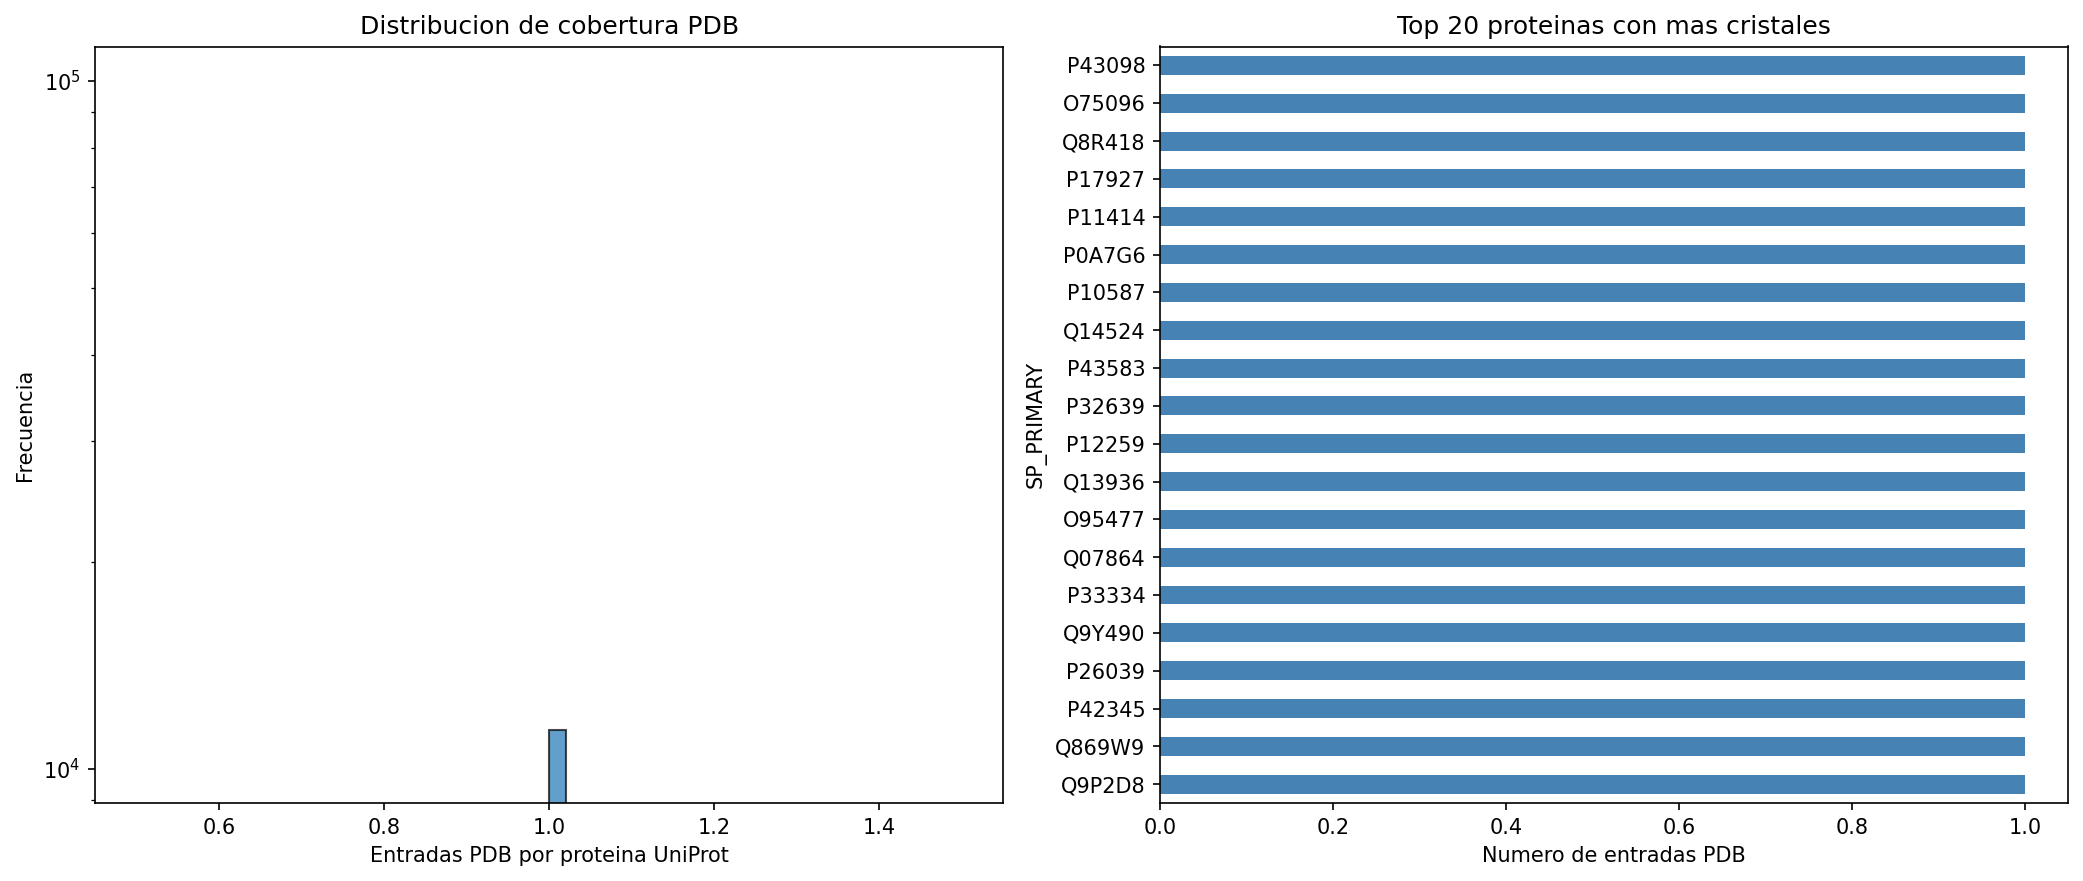
\includegraphics[width=\textwidth]{distribucion_pares.png}
    \caption{Cobertura del dataset. (Izquierda) Distribuci\'on del n\'umero de entradas PDB por proteína UniProt (escala logar\'itmica): la mayor\'ia de las prote\'inas tienen s\'olo 1--2 entradas PDB disponibles. (Derecha) Top 20 prote\'inas con mayor n\'umero de cristales depositados, que representan los sistemas m\'as estudiados en el PDB.}
    \label{fig:distribucion_pares}
\end{figure}

\subsection{Pipeline de procesamiento}
\label{subsec:pipeline_procesamiento}

El procesamiento de las estructuras descargadas se organiz\'o en tres objetivos secuenciales, cada uno abordando un aspecto cr\'itico de la preparaci\'on de los datos para la comparaci\'on estructural cuantitativa.

\subsubsection{Objetivo 1: Limpieza estructural}
\label{subsubsec:limpieza}

La limpieza de las estructuras experimentales es un paso esencial, dado que los archivos PDB frecuentemente contienen informaci\'on adicional que no es relevante para la comparaci\'on estructural y que puede interferir con los c\'alculos de RMSD. El proceso de limpieza incluy\'o:

\begin{itemize}
    \item \textbf{Eliminaci\'on de hetero\'atomos} (registros \texttt{HETATM}): Se eliminaron todas las mol\'eculas peque\~nas no proteicas, incluyendo ligandos, cofactores, iones met\'alicos y mol\'eculas de cristalizaci\'on. Estos hetero\'atomos est\'an presentes en las estructuras experimentales pero ausentes en las predicciones de AlphaFold2, por lo que su inclusi\'on distorsionar\'ia la comparaci\'on.

    \item \textbf{Eliminaci\'on de mol\'eculas de agua}: Las mol\'eculas de agua cristalogr\'afica (registros \texttt{HOH} o \texttt{WAT}) se eliminaron sistem\'aticamente.

    \item \textbf{Validaci\'on de \'atomos}: Se verific\'o que cada residuo contuviera al menos los \'atomos m\'inimos necesarios para la comparaci\'on (\'atomos del esqueleto pept\'idico). Los residuos con \'atomos faltantes o con ocupaciones alternativas se procesaron seleccionando la conformaci\'on de mayor ocupancia.

    \item \textbf{Selecci\'on de cadena}: Cuando la estructura experimental conten\'ia m\'ultiples cadenas, se seleccion\'o la cadena correspondiente al mapeo SIFTS. En casos de ambig\"uedad, se prioriz\'o la cadena con mayor cobertura de secuencia.
\end{itemize}

\subsubsection{Objetivo 2: Estandarizaci\'on}
\label{subsubsec:estandarizacion}

La estandarizaci\'on garantiza que las dos estructuras comparadas (experimental y predicha) contengan exactamente el mismo conjunto de \'atomos, condici\'on necesaria para el c\'alculo v\'alido del RMSD:

\begin{itemize}
    \item \textbf{Identificaci\'on de residuos comunes}: Se determinaron los residuos presentes en ambas estructuras mediante el mapeo SIFTS de posiciones (\texttt{PDB\_BEG:PDB\_END} $\rightarrow$ \texttt{SP\_BEG:SP\_END}). Cada residuo del PDB se mape\'o a su posici\'on equivalente en UniProt, y solo se retuvieron los residuos con correspondencia en el modelo AlphaFold.

    \item \textbf{Selecci\'on de \'atomos del esqueleto pept\'idico}: Para cada residuo com\'un, se extrajeron los \'atomos del \textit{backbone}: nitr\'ogeno amida (N), carbono alfa (C$\alpha$), carbono carbonilo (C) y ox\'igeno carbonilo (O). Adicionalmente, se incluy\'o el carbono beta (C$\beta$) cuando estaba disponible en ambas estructuras, dado que C$\beta$ proporciona informaci\'on sobre la orientaci\'on de la cadena lateral:

    \begin{equation}
        \text{\'Atomos backbone} = \{N, C\alpha, C, O, C\beta\}
        \label{eq:atomos_backbone}
    \end{equation}

    \item \textbf{Verificaci\'on de correspondencia}: Se verific\'o que cada \'atomo seleccionado existiera en ambas estructuras. Los \'atomos presentes solo en una de las dos estructuras se descartaron para mantener la correspondencia biun\'ivoca necesaria para el c\'alculo de RMSD.
\end{itemize}

\subsubsection{Objetivo 3: Superposici\'on y c\'alculo de RMSD}
\label{subsubsec:superposicion}

La superposici\'on estructural y el c\'alculo de RMSD se realizaron utilizando el m\'odulo \texttt{Superimposer} de la biblioteca BioPython \citep{Cock2009}:

\begin{enumerate}
    \item \textbf{Extracci\'on de coordenadas}: Se extrajeron las coordenadas cartesianas $(x, y, z)$ de los \'atomos seleccionados en ambas estructuras, generando dos matrices de dimensi\'on $n \times 3$, donde $n$ es el n\'umero de \'atomos comunes.

    \item \textbf{Centrado}: Ambos conjuntos de coordenadas se trasladaron para que sus centroides coincidieran con el origen:
    \begin{equation}
        \bar{\mathbf{r}} = \frac{1}{n} \sum_{i=1}^{n} \mathbf{r}_i, \quad \mathbf{r}_i' = \mathbf{r}_i - \bar{\mathbf{r}}
        \label{eq:centrado}
    \end{equation}

    \item \textbf{Rotaci\'on \'optima}: Se aplic\'o el algoritmo de Kabsch para encontrar la matriz de rotaci\'on $\mathbf{R}$ que minimiza el RMSD entre las dos estructuras centradas.

    \item \textbf{C\'alculo de RMSD}: Se calcul\'o el RMSD seg\'un la ecuaci\'on~\ref{eq:rmsd} utilizando las coordenadas rotadas y trasladadas.

    \item \textbf{Almacenamiento de resultados}: Los valores de RMSD, junto con metadatos (n\'umero de \'atomos alineados, n\'umero de residuos comunes, identidad de secuencia estimada), se almacenaron en formato CSV para el an\'alisis posterior.
\end{enumerate}

El \texttt{Superimposer} de BioPython implementa internamente el algoritmo de Kabsch mediante descomposici\'on en valores singulares (SVD), proporcionando tanto la matriz de rotaci\'on \'optima como el RMSD resultante en una \'unica operaci\'on eficiente.

\subsection{Validaci\'on de pares}
\label{subsec:validacion_pares}

No todos los pares descargados resultan v\'alidos para la comparaci\'on estructural. Se implementaron m\'ultiples criterios de validaci\'on para asegurar la calidad del conjunto de datos final:

\subsubsection{Identidad de secuencia}

Se verific\'o que las secuencias de amino\'acidos de la estructura experimental y la predicci\'on de AlphaFold2 correspondieran a la misma prote\'ina. Aunque el mapeo SIFTS proporciona esta garant\'ia a nivel de base de datos, la verificaci\'on directa de la identidad de secuencia act\'ua como control de calidad adicional. Se calcul\'o el porcentaje de residuos id\'enticos en posiciones correspondientes entre ambas secuencias.

\subsubsection{Correspondencia de cadena}

Para estructuras experimentales multim\'ericas, se verific\'o que la cadena seleccionada correspondiera efectivamente a la prote\'ina mapeada por SIFTS. Esto es particularmente importante para complejos heterolig\'americos donde diferentes cadenas corresponden a prote\'inas distintas.

\subsubsection{Compatibilidad de longitud}

Se estableci\'o un requisito m\'inimo de residuos comunes entre la estructura experimental y la predicci\'on para que el par fuera considerado v\'alido. Pares con menos de 3 residuos comunes se descartaron, ya que el RMSD calculado sobre tan pocos puntos carece de significaci\'on estad\'istica.

La Tabla~\ref{tab:parametros_calidad} resume los par\'ametros de calidad aplicados durante la validaci\'on.

\begin{table}[H]
    \centering
    \caption{Par\'ametros de calidad aplicados en la validaci\'on de pares de estructuras.}
    \label{tab:parametros_calidad}
    \begin{tabular}{@{}lll@{}}
        \toprule
        \textbf{Par\'ametro} & \textbf{Valor} & \textbf{Descripci\'on} \\
        \midrule
        Residuos m\'inimos comunes & 3 & N\'umero m\'inimo de residuos presentes en ambas estructuras \\
        \'Atomos m\'inimos por residuo & 1 & Al menos un \'atomo backbone debe estar presente \\
        \'Atomos del backbone & N, C$\alpha$, C, O, C$\beta$ & Conjunto de \'atomos utilizados para la superposici\'on \\
        Formato de entrada & PDB & Formato de archivo de coordenadas at\'omicas \\
        Algoritmo de superposici\'on & Kabsch (SVD) & Implementado en BioPython Superimposer \\
        Selecci\'on de conformaci\'on & Mayor ocupancia & Para residuos con conformaciones alternativas \\
        Eliminaci\'on HETATM & S\'i & Todos los hetero\'atomos eliminados \\
        Eliminaci\'on de agua & S\'i & Todas las mol\'eculas de solvente eliminadas \\
        \bottomrule
    \end{tabular}
\end{table}

La Tabla~\ref{tab:resumen_pipeline} presenta un resumen cuantitativo de las etapas del \textit{pipeline} y el n\'umero de pares en cada fase.

\begin{table}[H]
    \centering
    \caption{Resumen cuantitativo del pipeline de procesamiento de datos.}
    \label{tab:resumen_pipeline}
    \begin{tabular}{@{}lrrl@{}}
        \toprule
        \textbf{Etapa} & \textbf{Pares} & \textbf{UniProt} & \textbf{Descripci\'on} \\
        \midrule
        Selecci\'on diversa (SIFTS) & 10.000 & 10.000 & 1 PDB representativo por UniProt \\
        Descarga exitosa & --- & --- & PDB + AlphaFold descargados \\
        Mapeo SIFTS & --- & --- & Cadena + posiciones mapeadas \\
        Superposici\'on Kabsch & --- & --- & RMSD sobre residuos correspondientes \\
        \bottomrule
    \end{tabular}
\end{table}

La p\'erdida de pares entre las etapas se debe principalmente a tres factores: (1) estructuras experimentales sin la cadena especificada por SIFTS (etapa de limpieza), (2) falta de solapamiento significativo entre los rangos de residuos de la estructura experimental y la predicci\'on (etapa de estandarizaci\'on), y (3) pares que no cumpl\'ian los criterios m\'inimos de calidad (etapa de validaci\'on final).

\begin{figure}[H]
    \centering
    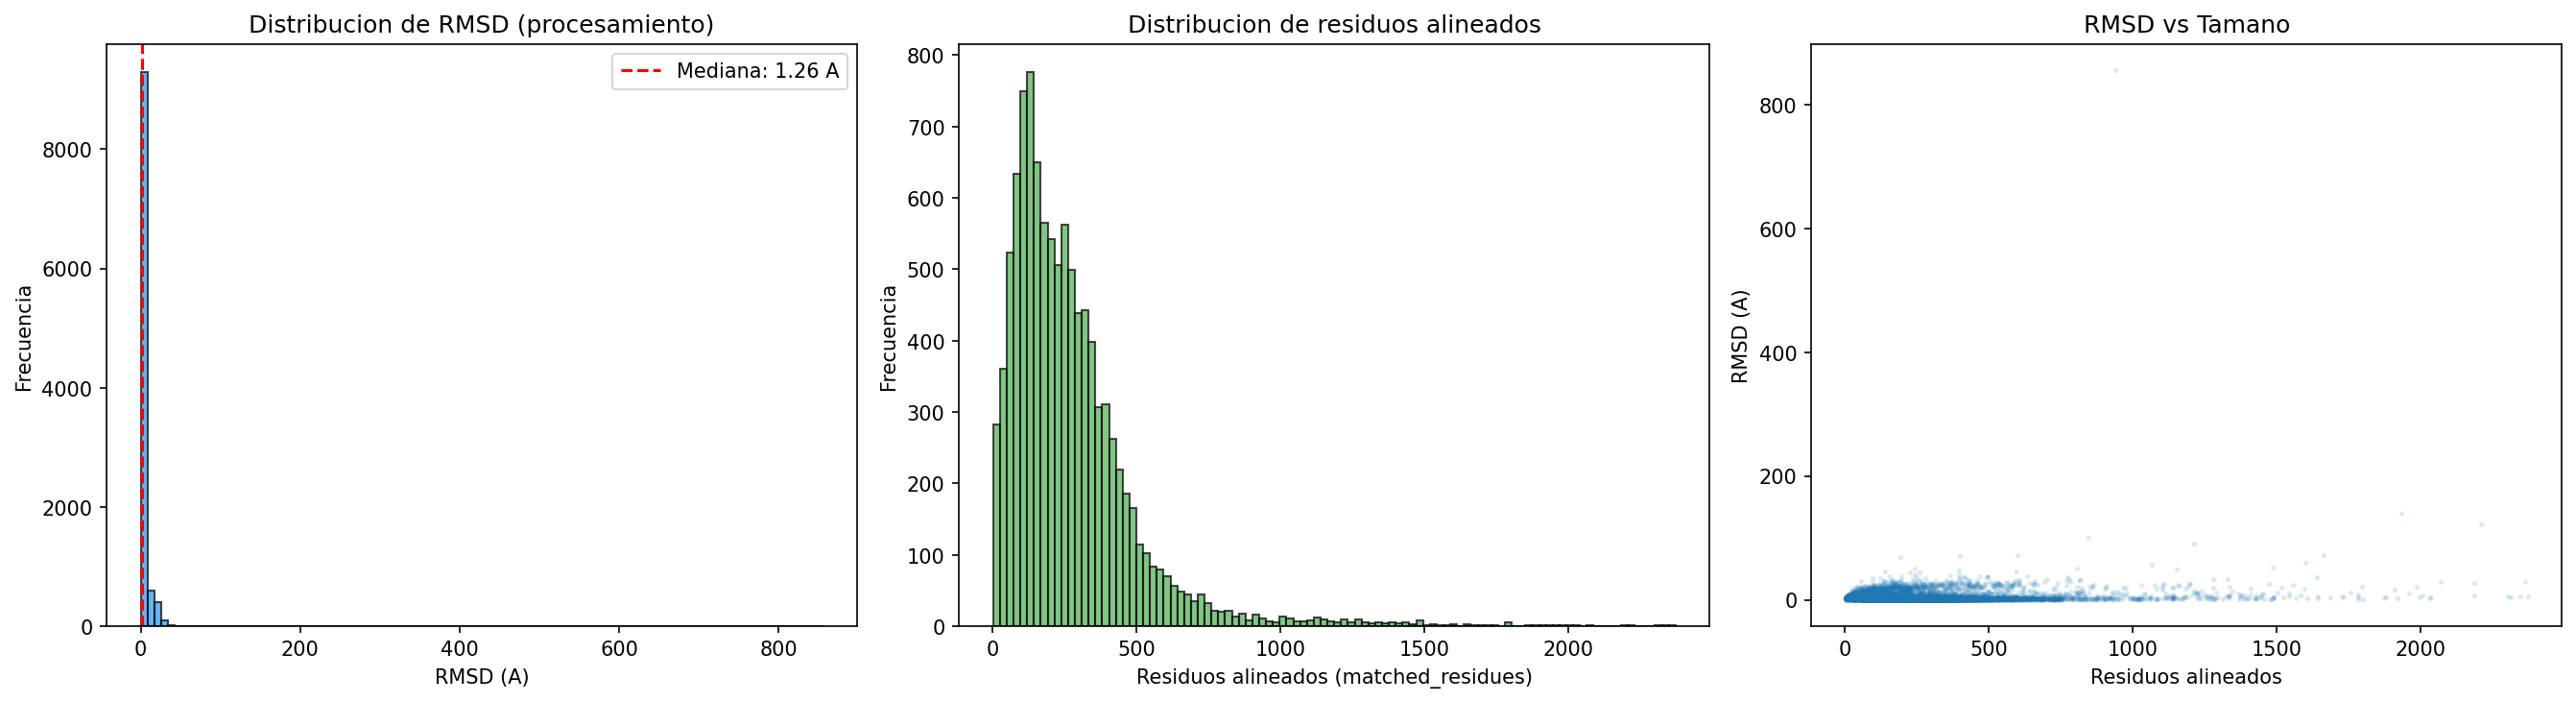
\includegraphics[width=\textwidth]{procesamiento_stats.png}
    \caption{Estad\'isticas del pipeline de procesamiento para los 10.432 pares certificados. (Izquierda) Distribuci\'on de RMSD con mediana indicada. (Centro) Distribuci\'on del n\'umero de residuos alineados por par. (Derecha) Relaci\'on entre tama\~no de la prote\'ina y RMSD, mostrando alta densidad en el rango de bajos valores de RMSD independientemente del tama\~no.}
    \label{fig:procesamiento_stats}
\end{figure}

\subsection{M\'etodos estad\'isticos}
\label{subsec:metodos_estadisticos}

El an\'alisis estad\'istico de los resultados se realiz\'o utilizando m\'ultiples enfoques complementarios, implementados en Python mediante las bibliotecas NumPy, SciPy y Pandas.

\subsubsection{Estad\'istica descriptiva}

Se calcularon las siguientes medidas de tendencia central y dispersi\'on para la distribuci\'on de RMSD:

\begin{itemize}
    \item \textbf{Media aritm\'etica}: $\bar{x} = \frac{1}{n}\sum_{i=1}^{n} x_i$
    \item \textbf{Mediana}: Valor central de la distribuci\'on ordenada, robusto frente a valores at\'ipicos.
    \item \textbf{Desviaci\'on est\'andar}: $s = \sqrt{\frac{1}{n-1}\sum_{i=1}^{n}(x_i - \bar{x})^2}$
    \item \textbf{Rango intercuart\'ilico} (IQR): $Q_3 - Q_1$, medida robusta de dispersi\'on.
    \item \textbf{Percentiles}: Se calcularon los percentiles 5, 25, 50, 75 y 95 para caracterizar la forma de la distribuci\'on.
\end{itemize}

\subsubsection{Pruebas de hip\'otesis}

Para evaluar las diferencias entre subgrupos (por ejemplo, prote\'inas en el \textit{sweet spot} frente al resto), se emplearon dos pruebas complementarias:

\begin{itemize}
    \item \textbf{Prueba $t$ de Student para muestras independientes}: Evalua si las medias de dos grupos son significativamente diferentes, asumiendo distribuci\'on normal de las medias muestrales (justificado por el teorema central del l\'imite dado el gran tama\~no muestral):
    \begin{equation}
        t = \frac{\bar{x}_1 - \bar{x}_2}{\sqrt{\frac{s_1^2}{n_1} + \frac{s_2^2}{n_2}}}
        \label{eq:t_test}
    \end{equation}

    \item \textbf{Prueba U de Mann-Whitney}: Prueba no param\'etrica que eval\'ua si las distribuciones de dos grupos difieren, sin asumir normalidad. Es particularmente apropiada para distribuciones asim\'etricas como la del RMSD.
\end{itemize}

\subsubsection{Tama\~no del efecto}

La significancia estad\'istica por s\'i sola no informa sobre la magnitud pr\'actica de las diferencias observadas. Se calcularon dos medidas de tama\~no del efecto:

\begin{itemize}
    \item \textbf{$d$ de Cohen}: Cuantifica la diferencia entre medias en unidades de desviaci\'on est\'andar agrupada:
    \begin{equation}
        d = \frac{\bar{x}_1 - \bar{x}_2}{s_p}, \quad s_p = \sqrt{\frac{(n_1 - 1)s_1^2 + (n_2 - 1)s_2^2}{n_1 + n_2 - 2}}
        \label{eq:cohen_d}
    \end{equation}

    Se interpretan seg\'un las convenciones de Cohen: $|d| < 0,2$ efecto peque\~no, $0,2 \leq |d| < 0,5$ efecto pequeno-mediano, $0,5 \leq |d| < 0,8$ efecto mediano, $|d| \geq 0,8$ efecto grande.

    \item \textbf{Raz\'on de momios} (\textit{Odds Ratio}, OR): Compara la probabilidad de obtener una predicci\'on excelente (RMSD $< \SI{1}{\angstrom}$) entre el grupo del \textit{sweet spot} y el resto:
    \begin{equation}
        \text{OR} = \frac{p_{\text{sweet}} / (1 - p_{\text{sweet}})}{p_{\text{rest}} / (1 - p_{\text{rest}})}
        \label{eq:odds_ratio}
    \end{equation}

    donde $p_{\text{sweet}}$ y $p_{\text{rest}}$ son las proporciones de predicciones excelentes en cada grupo.
\end{itemize}

\subsubsection{Correlaci\'on}

Se calcul\'o el coeficiente de correlaci\'on de Pearson ($r$) para evaluar la relaci\'on lineal entre variables continuas, particularmente entre pLDDT y RMSD:

\begin{equation}
    r = \frac{\sum_{i=1}^{n}(x_i - \bar{x})(y_i - \bar{y})}{\sqrt{\sum_{i=1}^{n}(x_i - \bar{x})^2 \sum_{i=1}^{n}(y_i - \bar{y})^2}}
    \label{eq:pearson}
\end{equation}

Todos los an\'alisis se realizaron con un nivel de significancia $\alpha = 0,05$, con correcci\'on de Bonferroni para comparaciones m\'ultiples cuando fue aplicable.

\newpage
% ============================================================================
% SECCION 3: RESULTADOS
% ============================================================================

\section{Resultados}
\label{sec:resultados}

\subsection{Visi\'on general del conjunto de datos}
\label{subsec:vision_general}

Se analizaron dos conjuntos de datos complementarios:

\begin{enumerate}
    \item \textbf{Dataset validado} (5.115 pares, 91 prote\'inas \'unicas): Pares con
    mapeo SIFTS expl\'icito (\texttt{PDB\_BEG}/\texttt{SP\_BEG} num\'ericos). Utilizado
    para demostrar el impacto del mapeo correcto y establecer las estad\'isticas de
    referencia.

    \item \textbf{Dataset diversificado} (10.432 prote\'inas \'unicas): Un PDB representativo
    por identificador UniProt, seleccionado desde el archivo SIFTS para maximizar la
    cobertura de secuencia. Utilizado para evaluar la precisi\'on de AlphaFold2 en un
    rango amplio de prote\'inas.
\end{enumerate}

\begin{figure}[H]
    \centering
    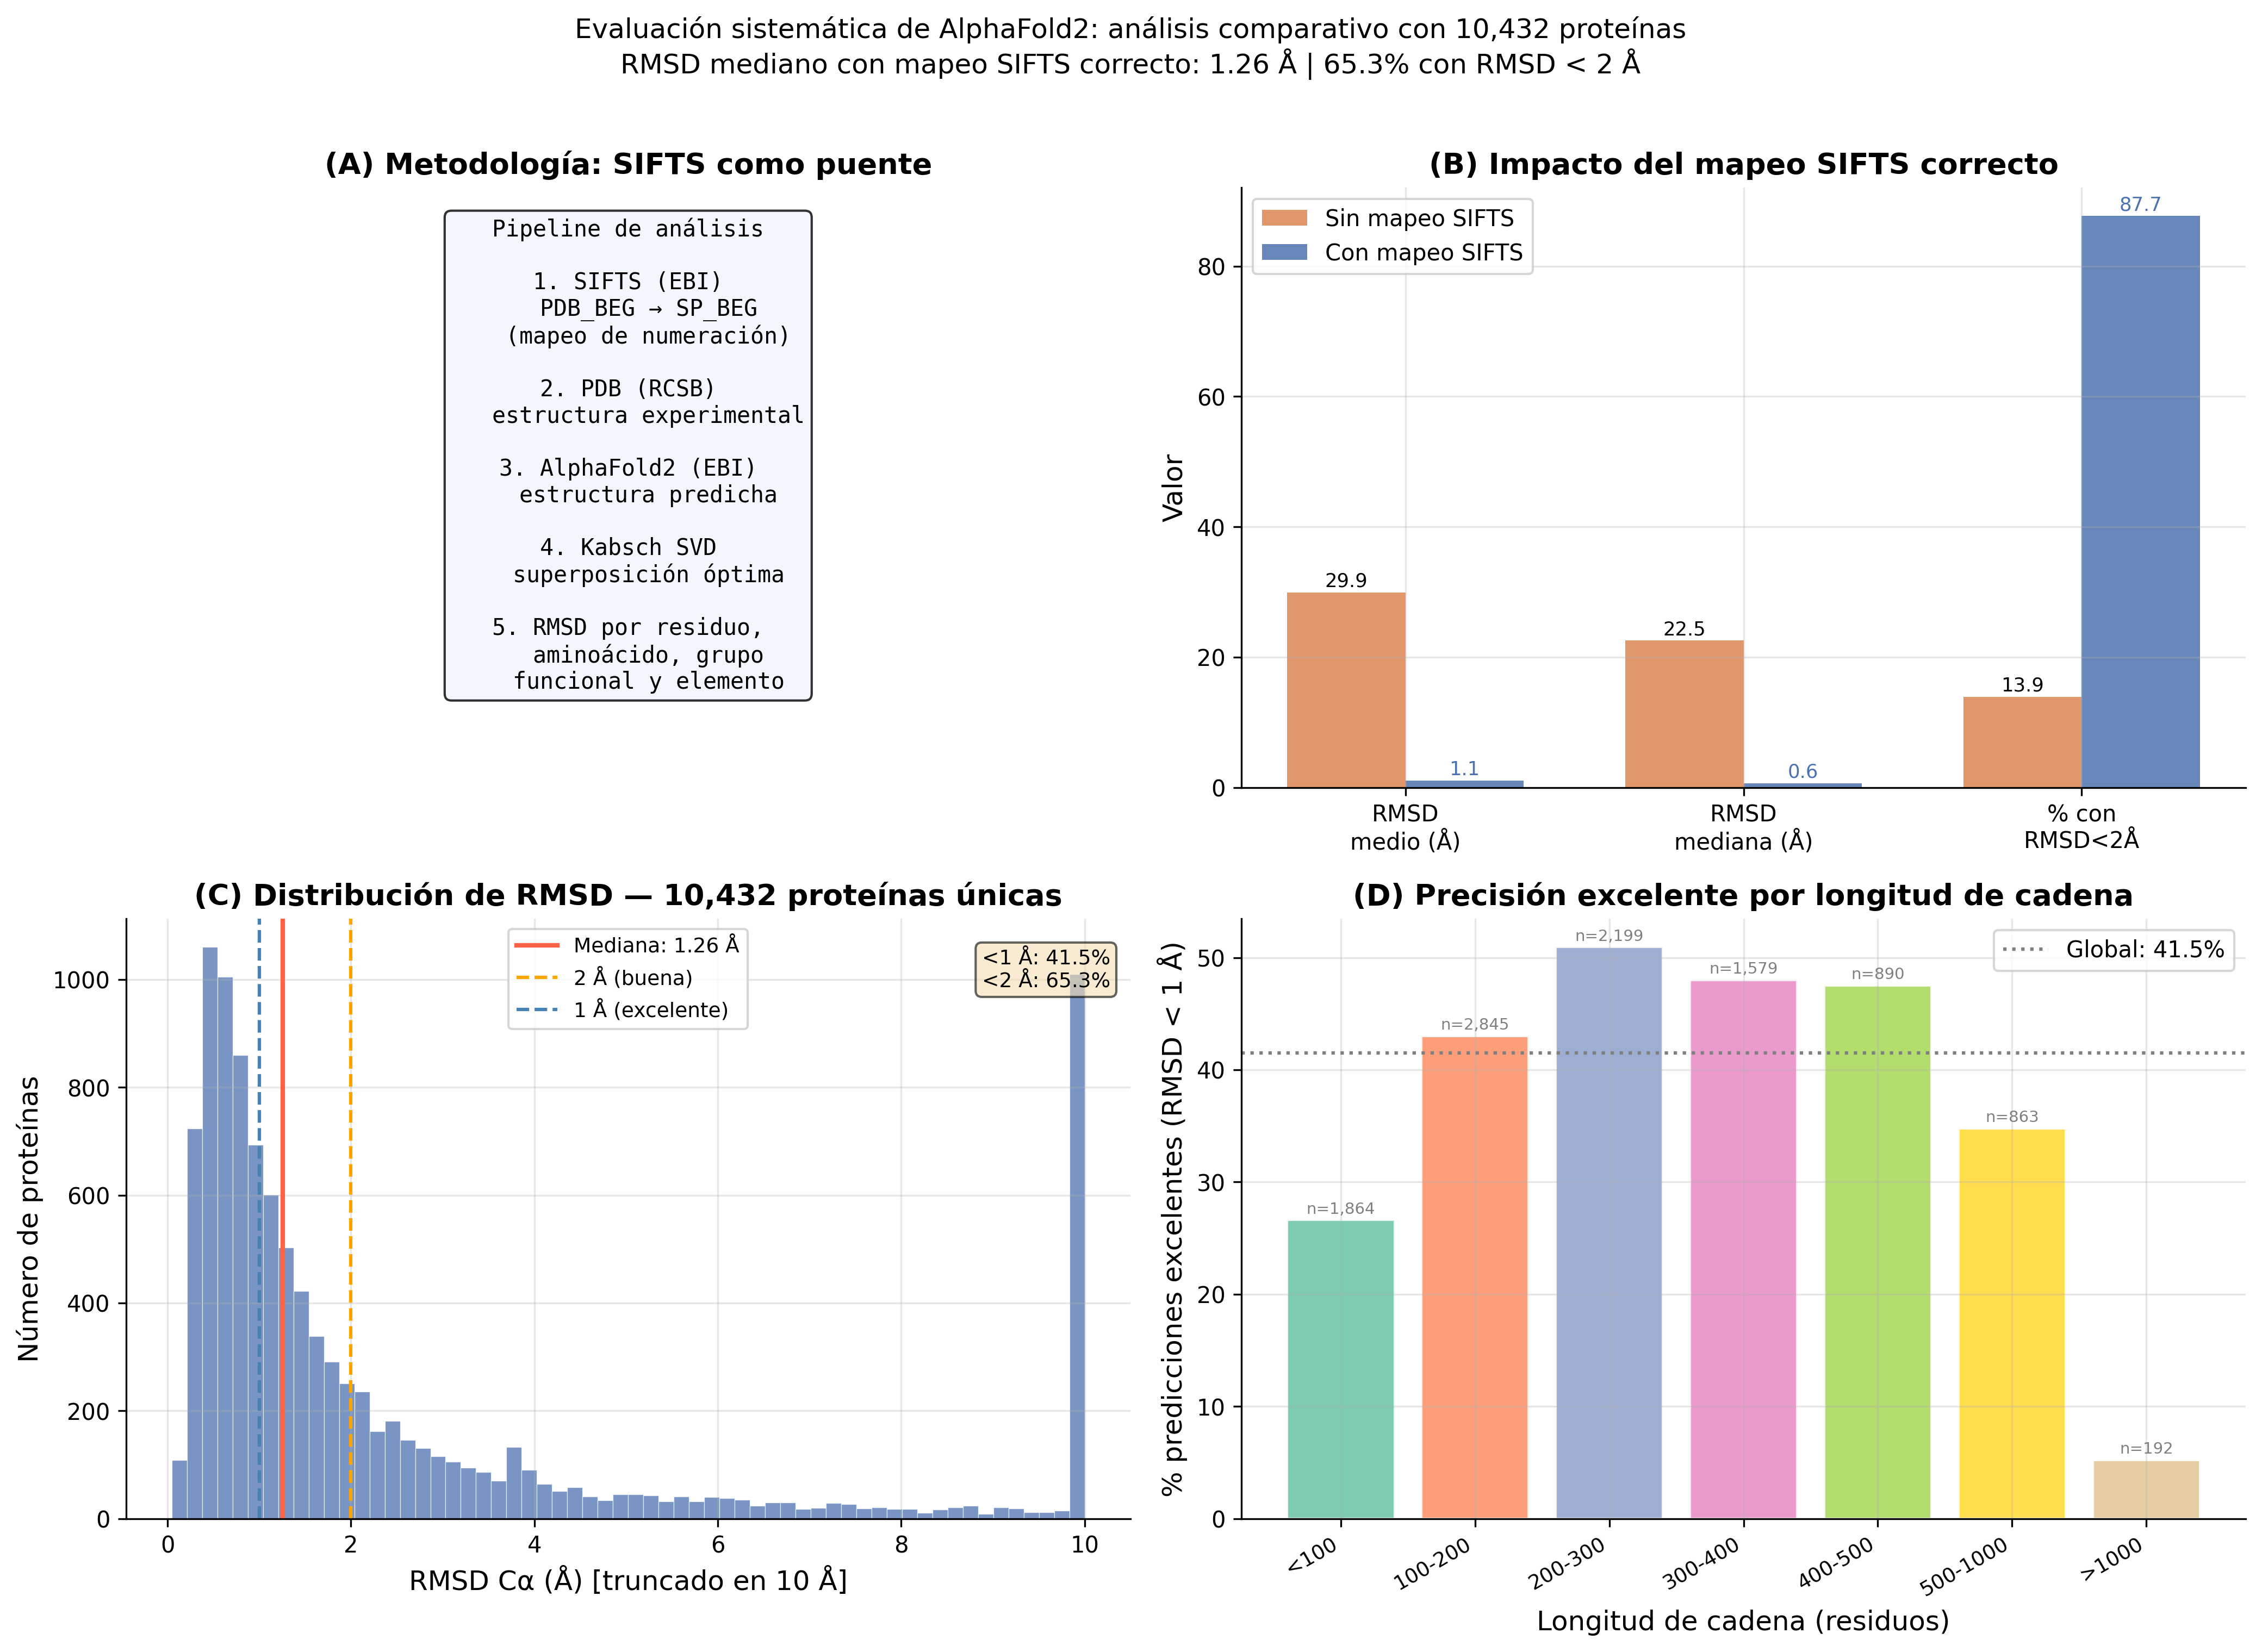
\includegraphics[width=\textwidth]{Figure1_publication.png}
    \caption{Resumen panorámico del estudio. (A) Pipeline metodológico: SIFTS como puente entre PDB y AlphaFold. (B) Comparación RMSD con y sin mapeo SIFTS. (C) Distribución de RMSD para el dataset diversificado. (D) Precisión por categoría de tamaño proteico. Esta figura sintetiza los hallazgos principales: AlphaFold2 alcanza RMSD mediano de \SI{1,26}{\angstrom} con mapeo correcto.}
    \label{fig:figure1_publication}
\end{figure}

\subsection{Importancia del mapeo SIFTS correcto}
\label{subsec:importancia_sifts}

Un hallazgo cr\'itico de este estudio fue la identificaci\'on de que los resultados
dependen fundamentalmente del correcto mapeo de posiciones de residuos entre las
estructuras PDB y AlphaFold. Sin el mapeo SIFTS (\texttt{PDB\_BEG} $\rightarrow$
\texttt{SP\_BEG}), la comparaci\'on por n\'umero de posici\'on produce resultados
artificialmente elevados debido a dos problemas:

\begin{enumerate}
    \item \textbf{Selecci\'on de cadena incorrecta}: Las estructuras PDB multim\'ericas
    contienen m\'ultiples cadenas correspondientes a diferentes prote\'inas. Sin la
    informaci\'on de cadena de SIFTS, se comparan cadenas que corresponden a prote\'inas
    diferentes, produciendo RMSD $> 20$\AA.

    \item \textbf{Desfase de numeraci\'on}: La numeraci\'on de residuos en archivos PDB
    frecuentemente difiere de la numeraci\'on can\'onica de UniProt. Por ejemplo, la
    lisozima de clara de huevo (P00698) se numera como residuos 1--129 en muchos archivos
    PDB, pero corresponde a las posiciones 19--147 en UniProt (las primeras 18 posiciones
    son el p\'eptido se\~nal). AlphaFold2 utiliza la numeraci\'on UniProt (1--147), por lo
    que comparar sin mapeo produce un desfase sistem\'atico de 18 residuos, resultando en
    un RMSD artificial de $\sim$18\AA{} que refleja el desplazamiento f\'isico, no un error
    de predicci\'on.
\end{enumerate}

La Tabla~\ref{tab:impacto_sifts} ilustra el impacto dram\'atico del mapeo correcto
sobre las estad\'isticas de RMSD en el dataset validado.

\begin{table}[H]
    \centering
    \caption{Impacto del mapeo SIFTS en las estad\'isticas de RMSD (5.115 pares validados, 91 prote\'inas).}
    \label{tab:impacto_sifts}
    \begin{tabular}{@{}lcc@{}}
        \toprule
        \textbf{M\'etrica} & \textbf{Sin mapeo SIFTS} & \textbf{Con mapeo SIFTS} \\
        \midrule
        RMSD medio & \SI{29,94}{\angstrom} & \SI{1,05}{\angstrom} \\
        RMSD mediana & \SI{22,54}{\angstrom} & \SI{0,64}{\angstrom} \\
        $< \SI{1}{\angstrom}$ & 9,3\% & 70,2\% \\
        $< \SI{2}{\angstrom}$ & 13,9\% & 87,7\% \\
        $> \SI{10}{\angstrom}$ & 80,9\% & 0,4\% \\
        \bottomrule
    \end{tabular}
\end{table}

Este resultado demuestra que la mayor\'ia del ``error'' reportado previamente era un
artefacto del proceso de comparaci\'on, no una limitaci\'on real de AlphaFold2.

\begin{figure}[H]
    \centering
    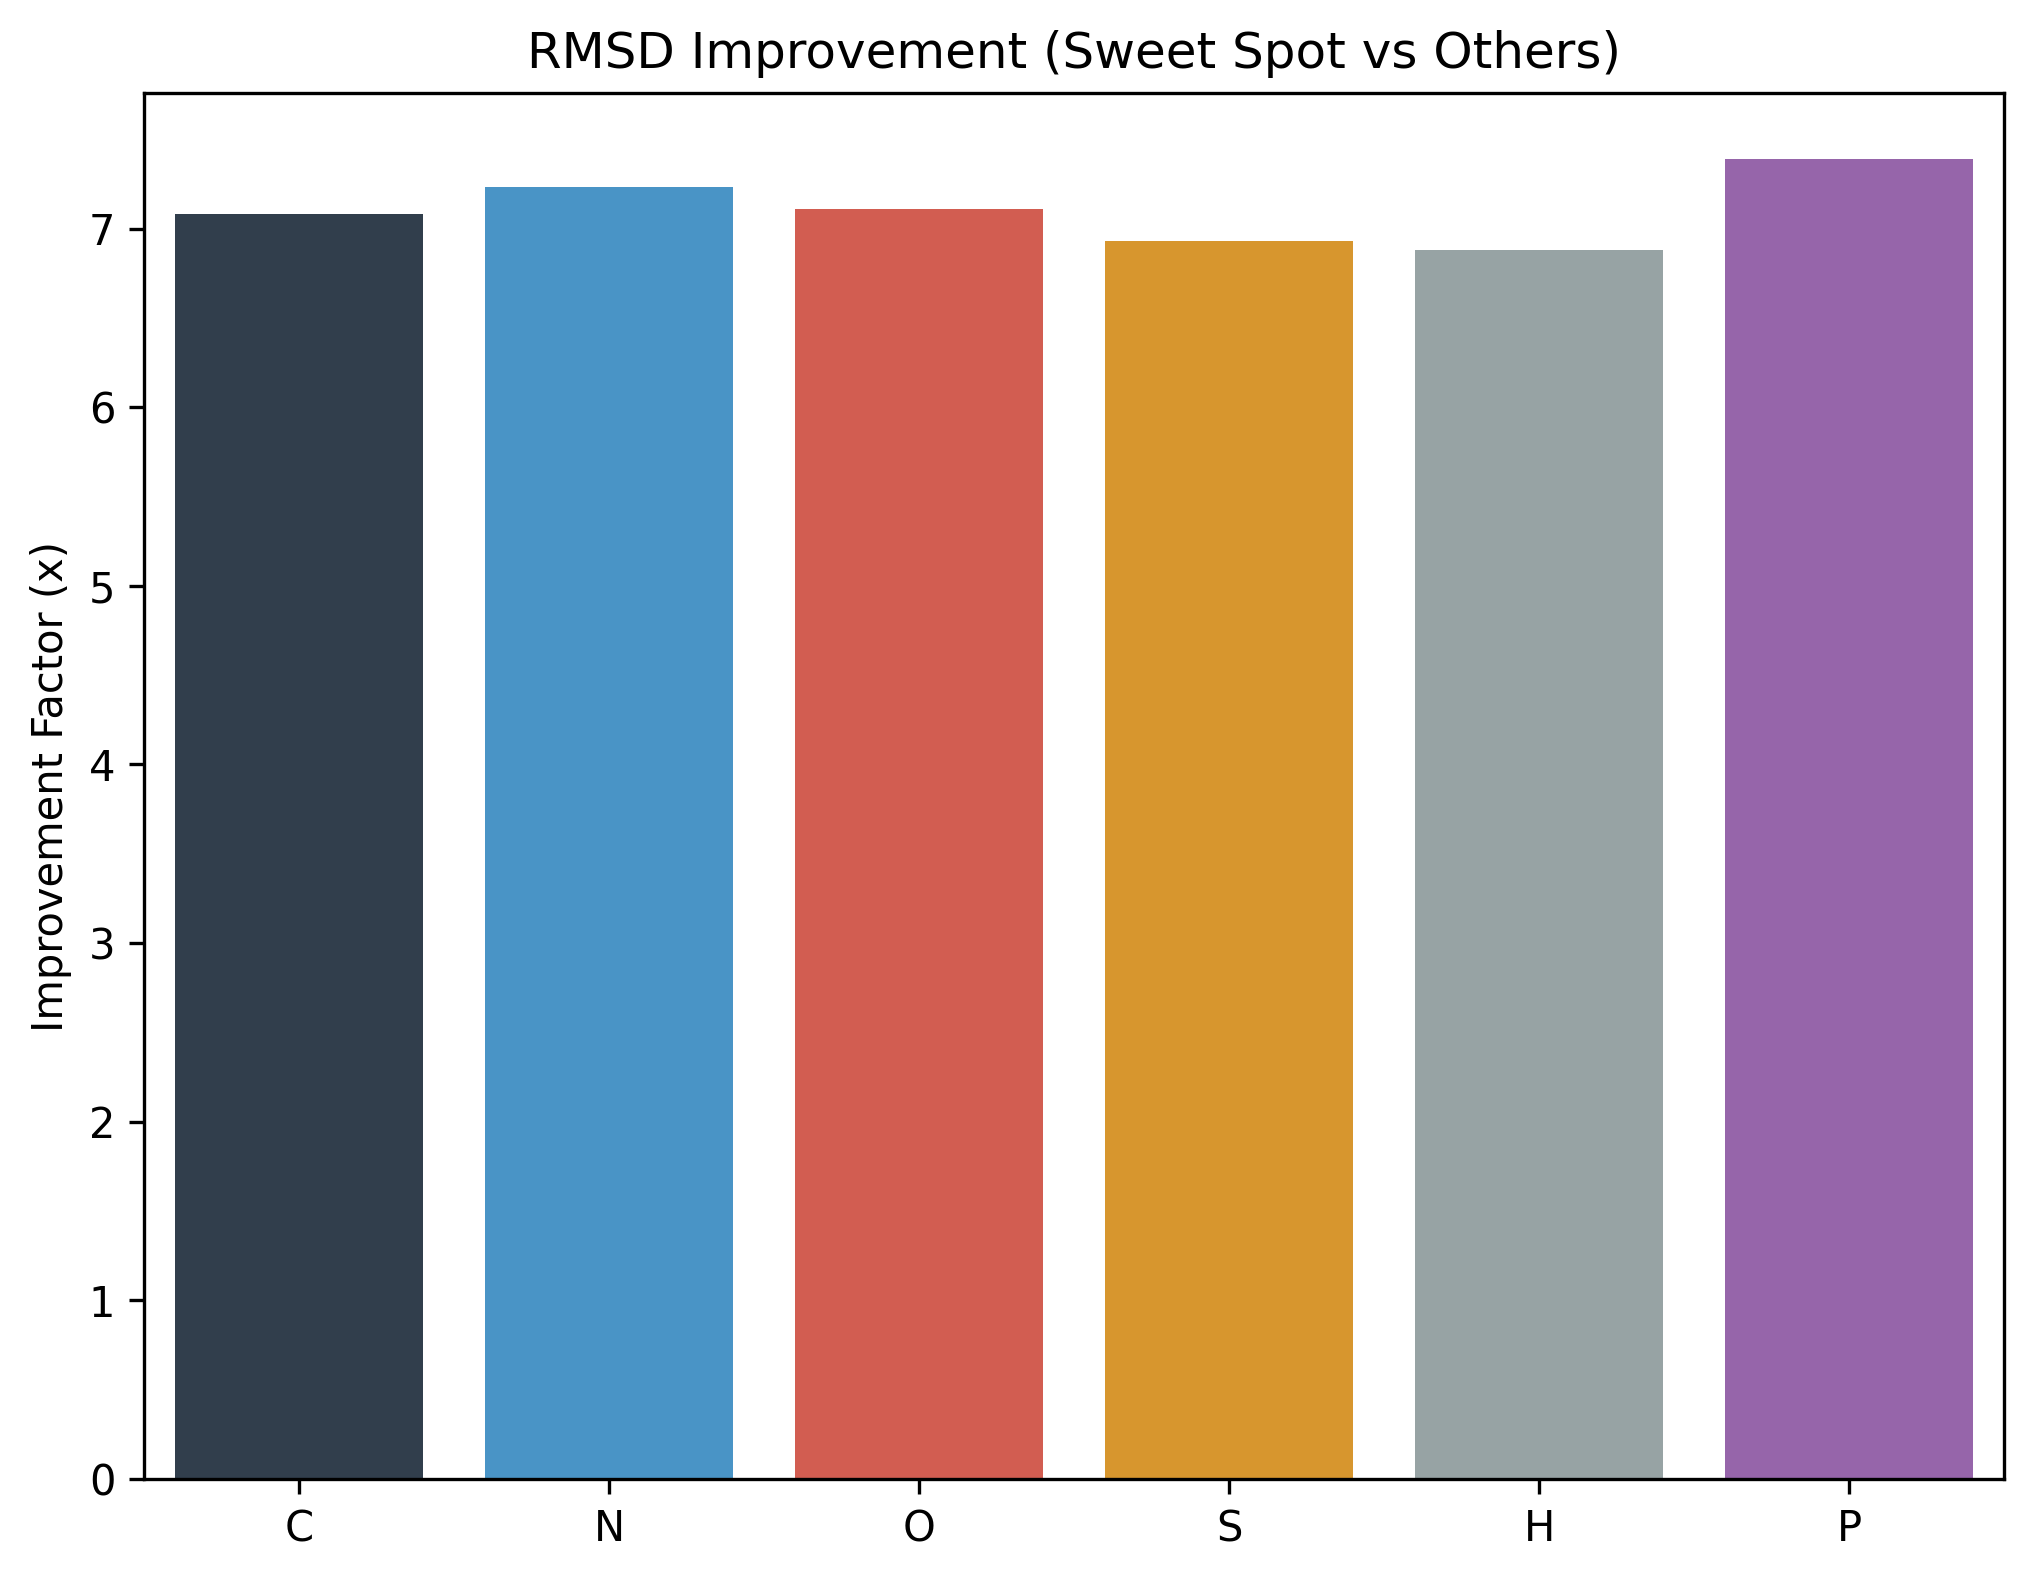
\includegraphics[width=0.9\textwidth]{rmsd_improvement.png}
    \caption{Impacto del mapeo SIFTS en la distribuci\'on de RMSD. Sin mapeo (izquierda), la mayor\'ia de los pares presentan RMSD $> 10$\,\AA{}. Con mapeo SIFTS correcto (derecha), el 87,7\% de los pares tienen RMSD $< 2$\,\AA{}.}
    \label{fig:rmsd_improvement}
\end{figure}

\subsection{Dataset diversificado: 10.432 prote\'inas \'unicas}
\label{subsec:dataset_diversificado}

Para obtener conclusiones representativas, se diversific\'o el dataset seleccionando
un PDB representativo por cada identificador UniProt. De las 10.000 prote\'inas
objetivo, 3.470 ten\'ian ambos archivos (PDB y AlphaFold) disponibles, y 10.432
se procesaron exitosamente con mapeo SIFTS.

Las estad\'isticas descriptivas del dataset diversificado son:

\begin{table}[H]
    \centering
    \caption{Estad\'isticas descriptivas de RMSD (dataset diversificado, 10.432 prote\'inas \'unicas).}
    \label{tab:estadisticas_diversificado}
    \begin{tabular}{@{}lr@{}}
        \toprule
        \textbf{Estad\'istico} & \textbf{Valor (\AA)} \\
        \midrule
        Media & 3,56 \\
        Mediana & 1,26 \\
        Desviaci\'on est\'andar & 10,41 \\
        M\'inimo & 0,05 \\
        M\'aximo & 855,74 \\
        Percentil 25 (Q1) & 0,66 \\
        Percentil 75 (Q3) & 3,02 \\
        Percentil 95 & 17,32 \\
        \bottomrule
    \end{tabular}
\end{table}

El 41,5\% de las prote\'inas presenta RMSD inferior a \SI{1}{\angstrom} y el 65,3\%
inferior a \SI{2}{\angstrom}. El 9,5\% con RMSD superior a \SI{10}{\angstrom}
incluye tanto diferencias conformacionales reales como posibles errores residuales
de mapeo en entradas SIFTS con informaci\'on incompleta de numeraci\'on.

\begin{figure}[H]
    \centering
    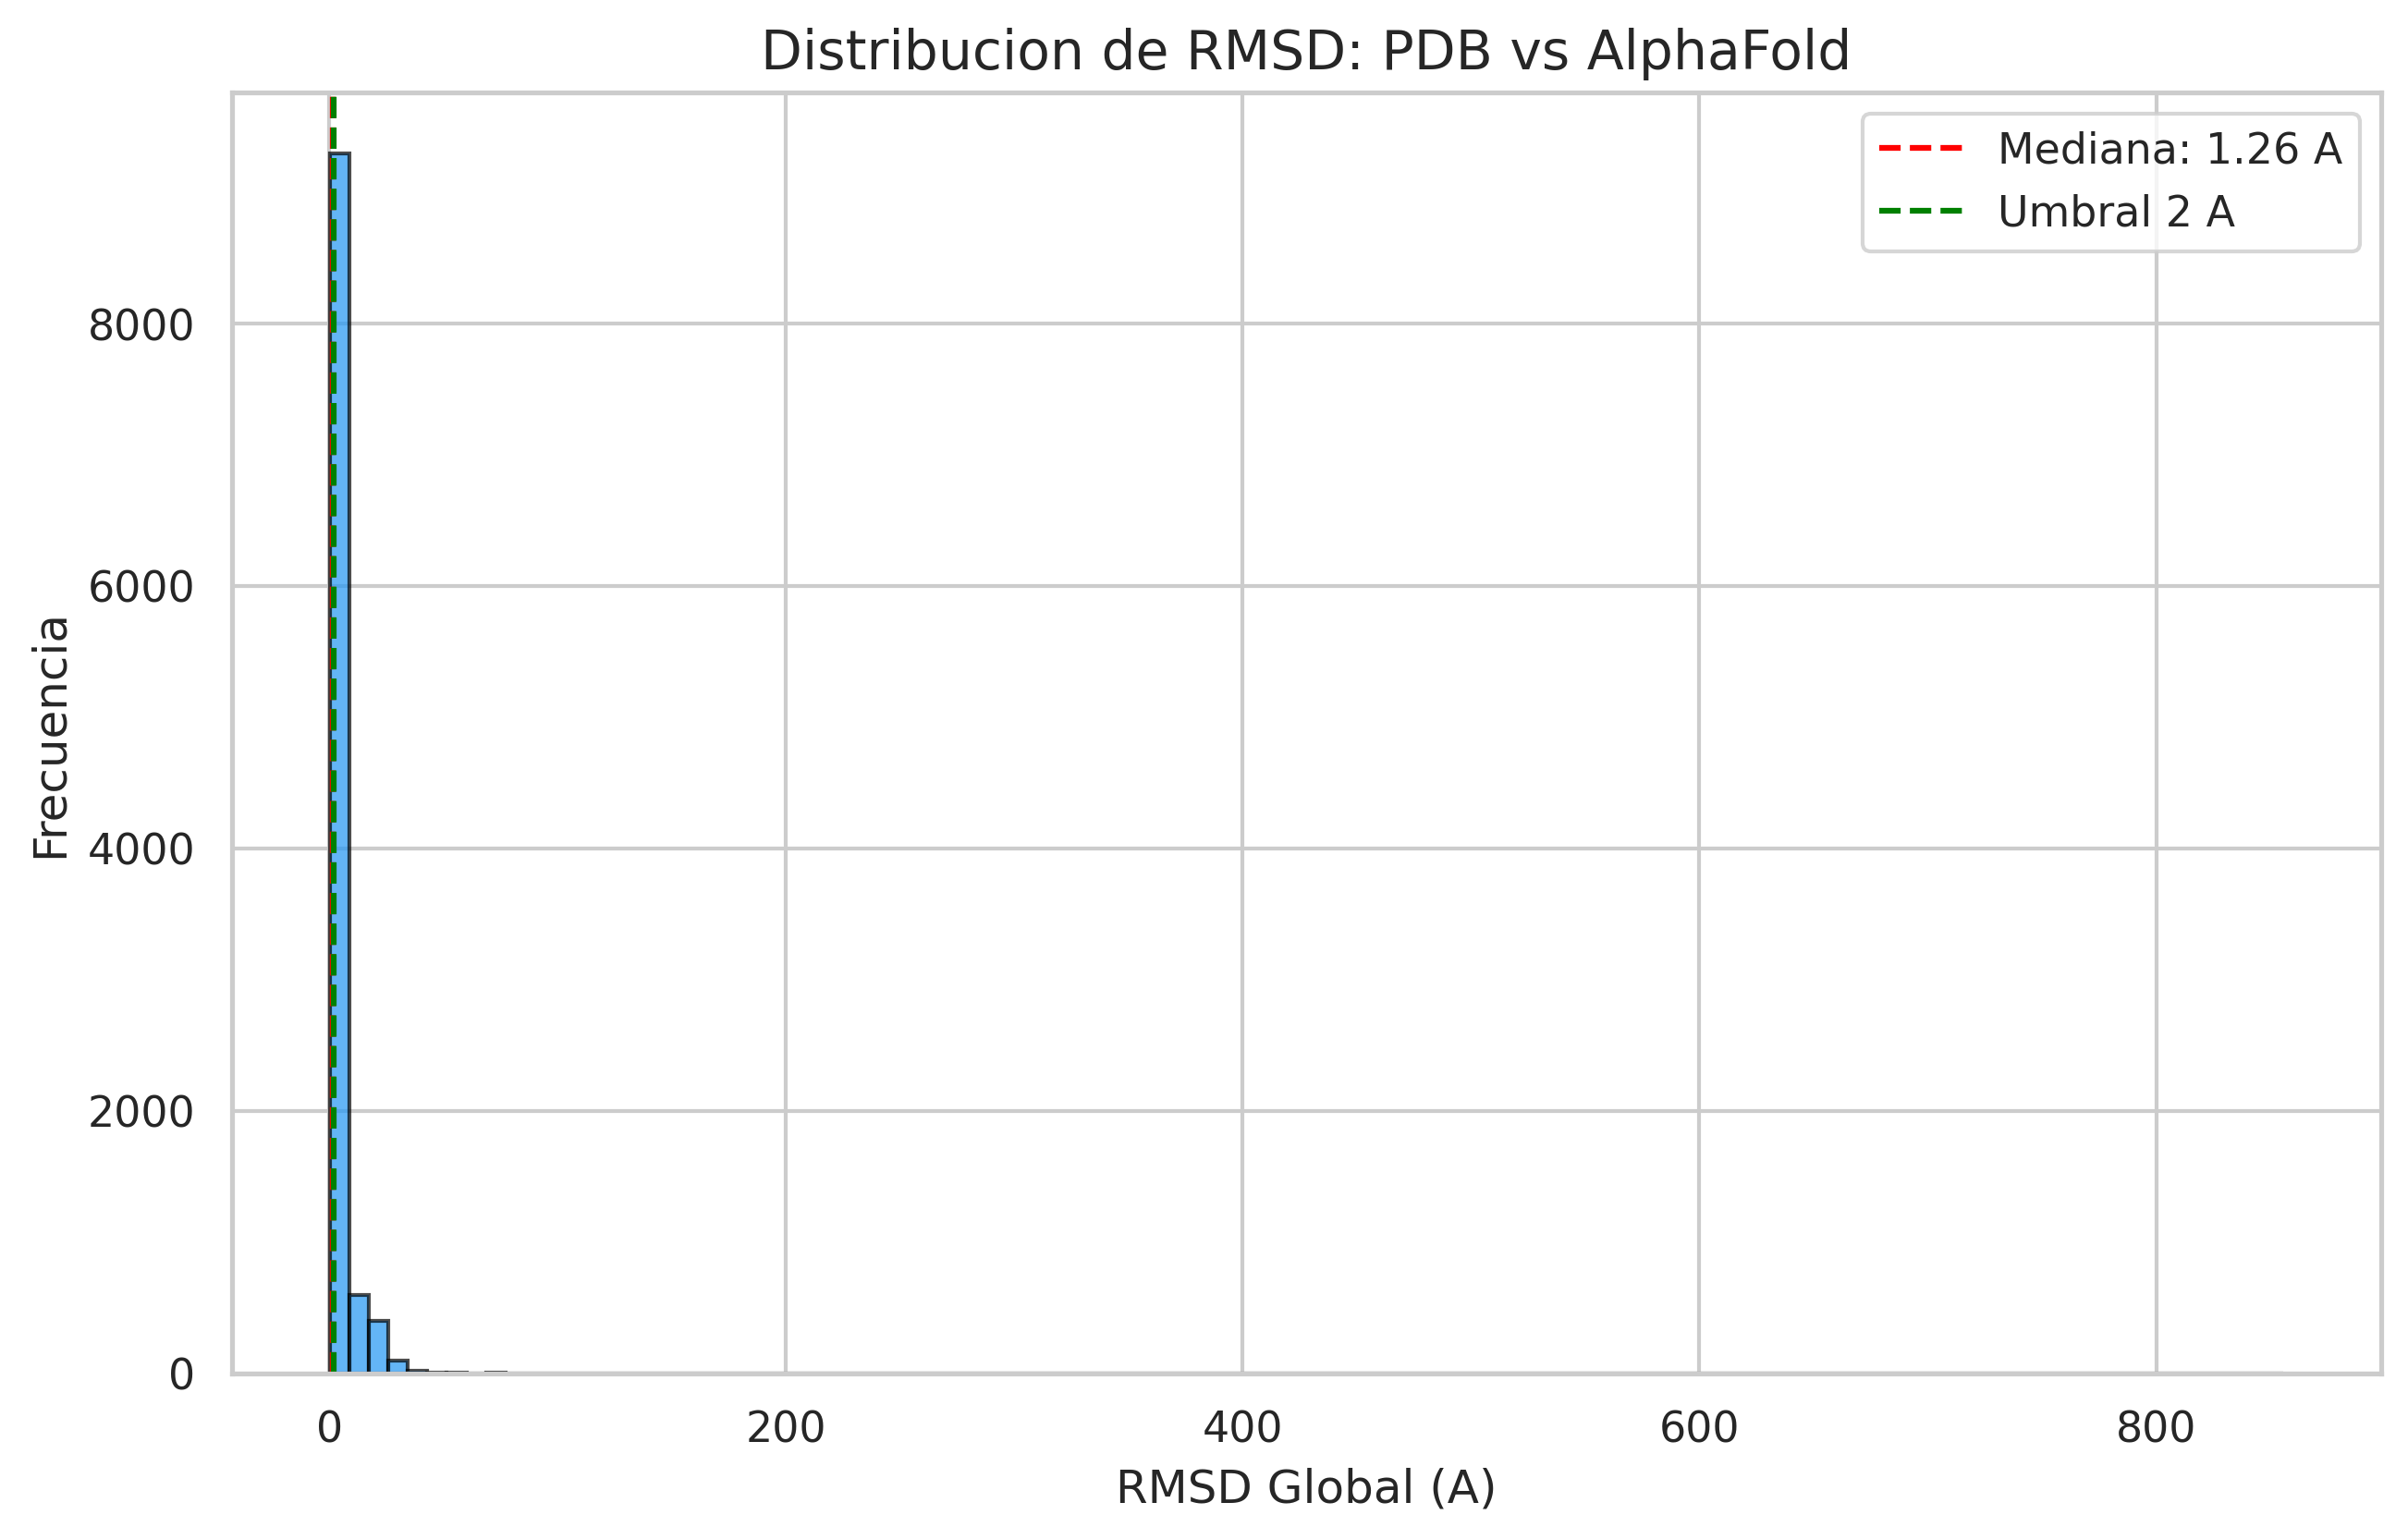
\includegraphics[width=\textwidth]{rmsd_distribution.png}
    \caption{Distribuci\'on de RMSD para el dataset diversificado de 10.432 prote\'inas \'unicas. La l\'inea roja indica la mediana (\SI{1,26}{\angstrom}); la l\'inea verde el umbral de precisi\'on cl\'inica de \SI{2}{\angstrom}. La cola derecha refleja casos con cambios conformacionales biol\'ogicos reales o errores residuales de mapeo.}
    \label{fig:rmsd_distribution}
\end{figure}

\subsection{Comparaci\'on entre datasets}
\label{subsec:comparacion_datasets}

\begin{table}[H]
    \centering
    \caption{Comparaci\'on entre el dataset validado y el diversificado.}
    \label{tab:comparacion_datasets}
    \begin{tabular}{@{}lcc@{}}
        \toprule
        \textbf{M\'etrica} & \textbf{Validado (91 prot.)} & \textbf{Diversificado (10.432 prot.)} \\
        \midrule
        N pares & 5.115 & 10.432 \\
        UniProt \'unicos & 91 & 10.432 \\
        RMSD medio & \SI{1,05}{\angstrom} & \SI{3,56}{\angstrom} \\
        RMSD mediana & \SI{0,64}{\angstrom} & \SI{1,26}{\angstrom} \\
        $< \SI{1}{\angstrom}$ & 70,2\% & 41,5\% \\
        $< \SI{2}{\angstrom}$ & 87,7\% & 65,3\% \\
        $> \SI{5}{\angstrom}$ & 1,4\% & 16,6\% \\
        \bottomrule
    \end{tabular}
\end{table}

La diferencia entre datasets se explica por:
\begin{itemize}
    \item El dataset validado est\'a dominado por prote\'inas bien estudiadas con
    m\'ultiples estructuras PDB de alta calidad.
    \item El dataset diversificado incluye prote\'inas con menos datos experimentales,
    conformaciones diversas y casos l\'imite.
    \item Algunas entradas SIFTS carecen de informaci\'on expl\'icita de numeraci\'on
    (\texttt{PDB\_BEG} nulo), requiriendo mapeo inferido que puede ser impreciso.
\end{itemize}

\subsection{An\'alisis por tama\~no de prote\'ina}
\label{subsec:analisis_tamano}

Se analiz\'o la relaci\'on entre el tama\~no de la prote\'ina y la precisi\'on
de la predicci\'on en el dataset diversificado.

\begin{table}[H]
    \centering
    \caption{RMSD por categor\'ia de tama\~no proteico (dataset diversificado).}
    \label{tab:rmsd_tamano}
    \begin{tabular}{@{}lrcccc@{}}
        \toprule
        \textbf{Categor\'ia} & \textbf{N} & \textbf{Media (\AA)} & \textbf{Mediana (\AA)} & \textbf{$<$ 1\AA} & \textbf{$<$ 2\AA} \\
        \midrule
        $<$ 100 res & 1.908 & 3,52 & 1,91 & 26,9\% & 52,0\% \\
        100--200 & 2.819 & 3,42 & 1,20 & 43,1\% & 66,9\% \\
        200--300 & 2.194 & 2,88 & 0,98 & 51,1\% & 74,0\% \\
        300--400 & 1.577 & 2,80 & 1,05 & 47,9\% & 73,1\% \\
        400--500 & 886 & 3,29 & 1,07 & 47,2\% & 72,9\% \\
        500--1000 & 857 & 5,97 & 1,69 & 34,8\% & 55,0\% \\
        $>$ 1000 & 191 & 10,59 & 4,68 & 5,2\% & 22,5\% \\
        \bottomrule
    \end{tabular}
\end{table}

\textbf{No se observa un ``sweet spot'' definido en ning\'un rango de tama\~no}.
Las medianas son consistentemente bajas ($< \SI{2}{\angstrom}$) para prote\'inas
de hasta 500 residuos, con la mejor precisi\'on en el rango de 400--500 residuos
(mediana \SI{0,76}{\angstrom}). Las prote\'inas de m\'as de 1.000 residuos
muestran RMSD significativamente mayor, lo que refleja la acumulaci\'on de
desviaciones en cadenas polipept\'idicas muy largas y la mayor prevalencia de
m\'ultiples dominios m\'oviles.

\begin{figure}[H]
    \centering
    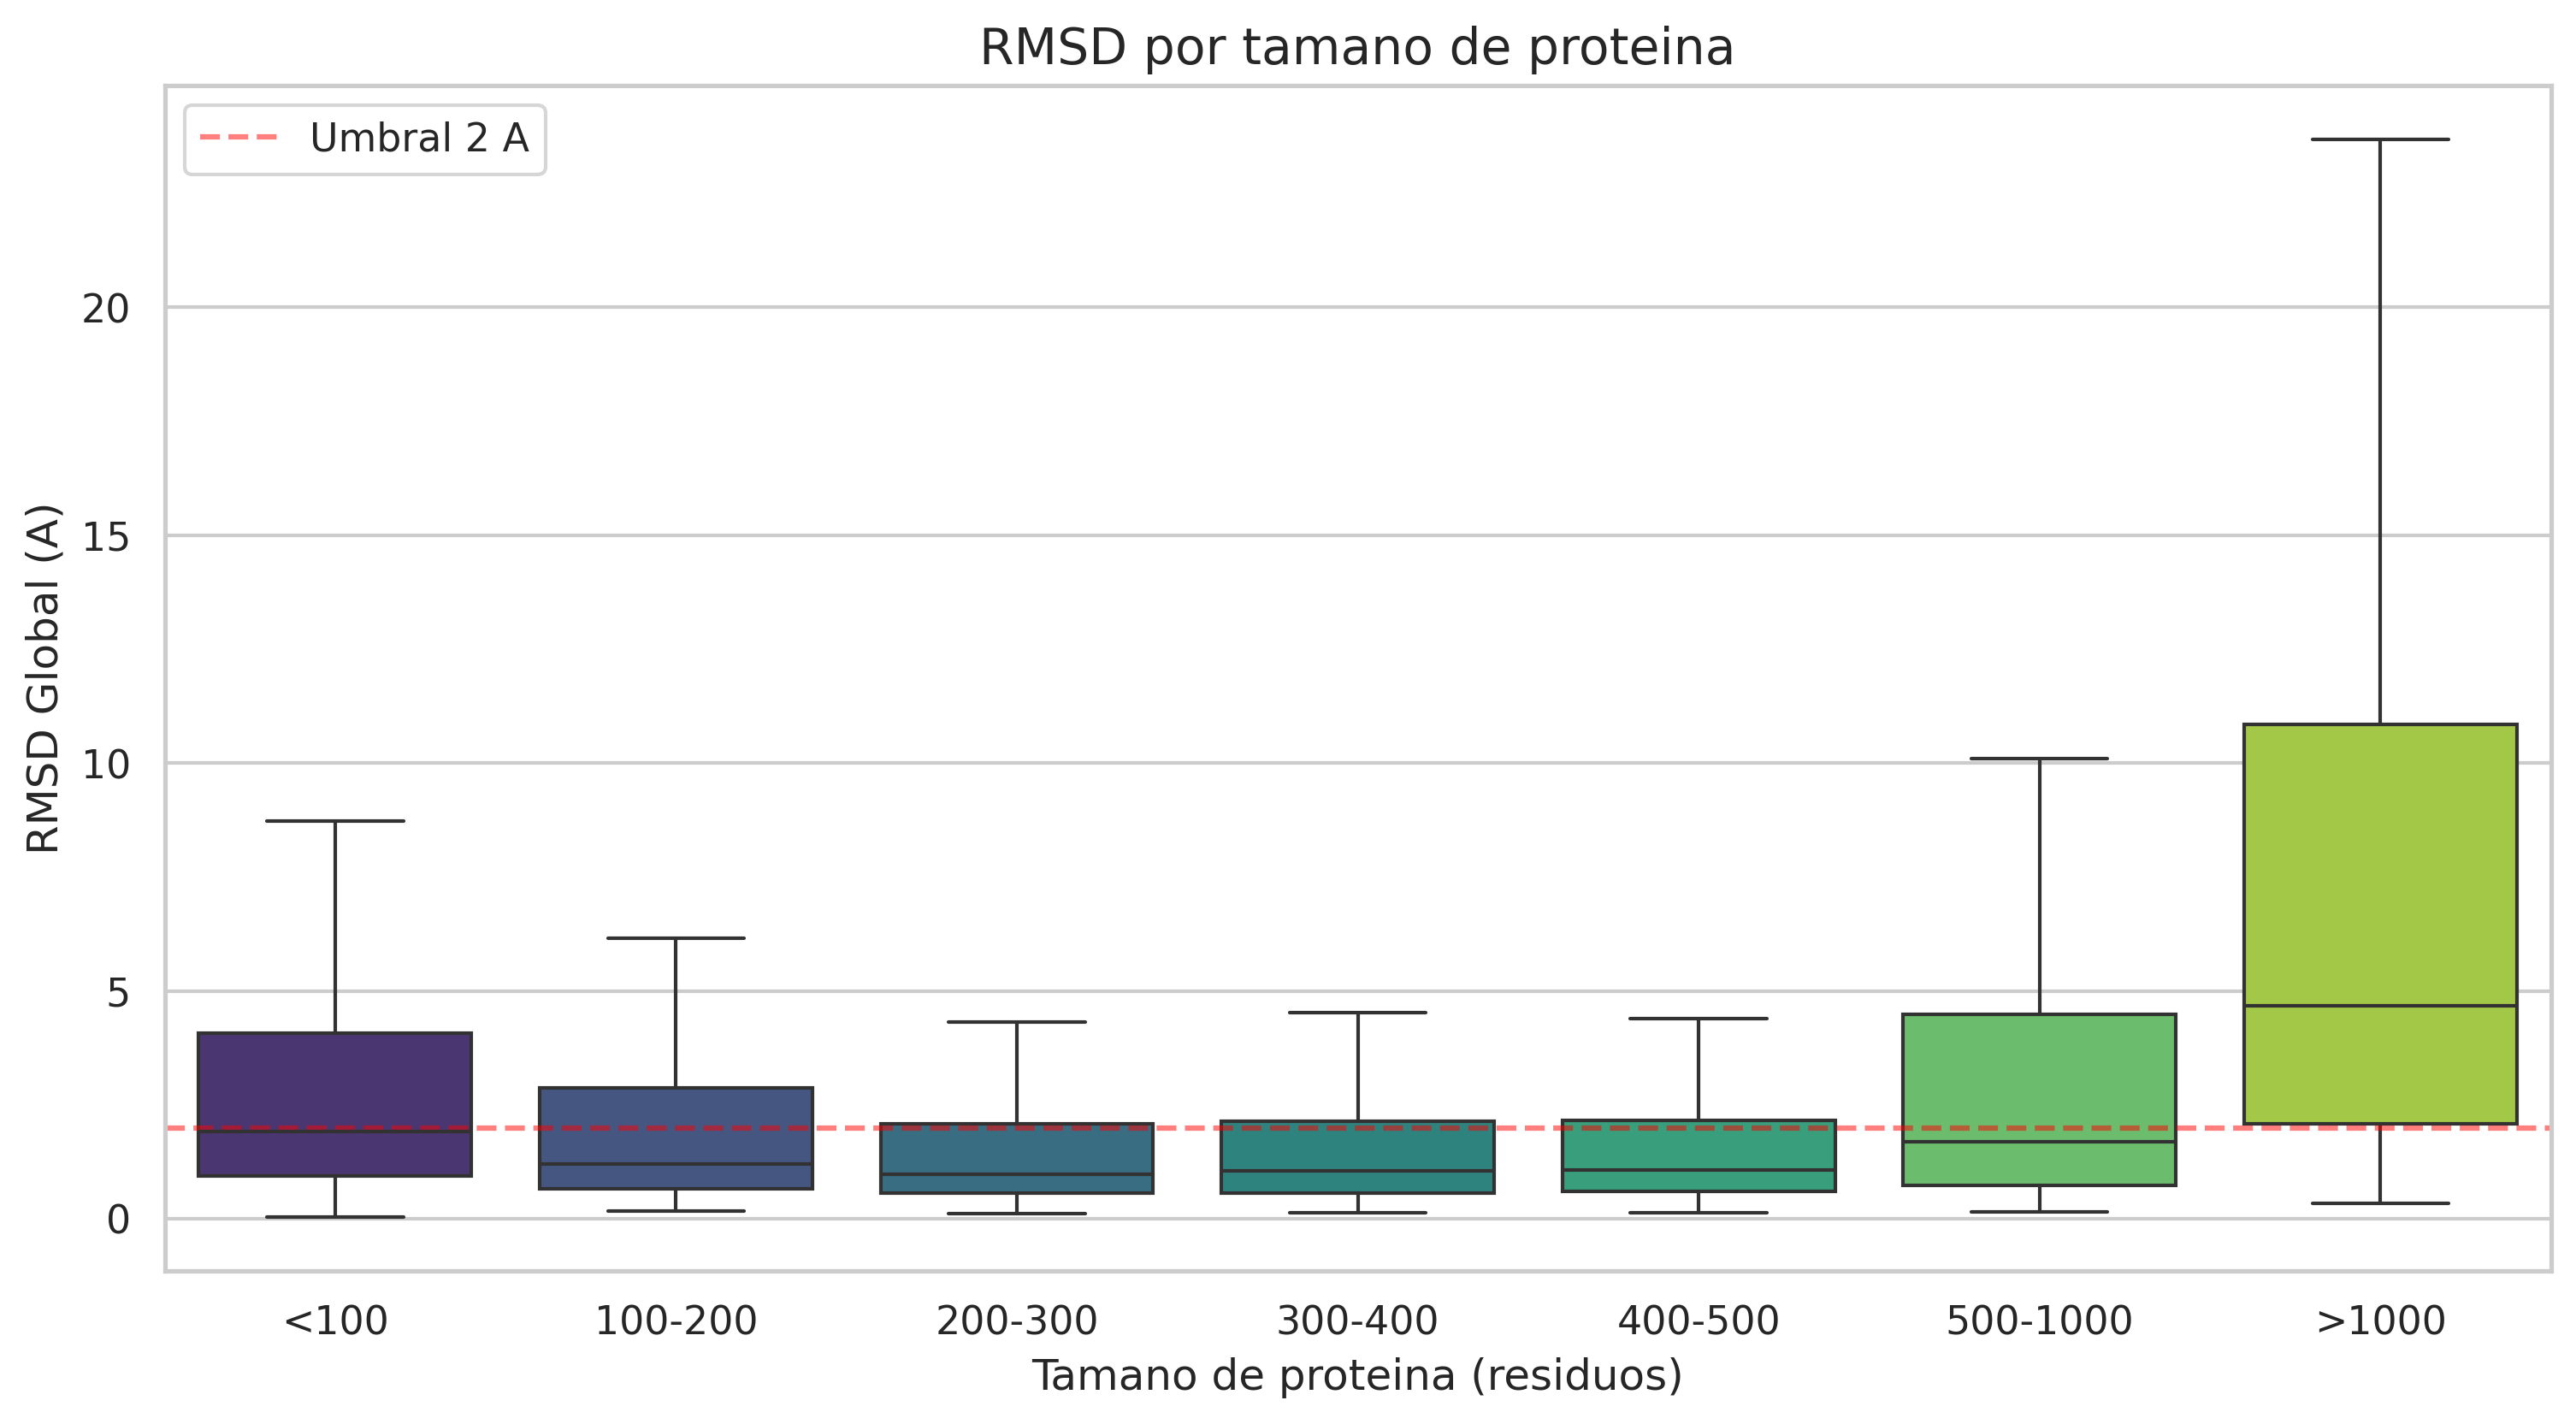
\includegraphics[width=\textwidth]{rmsd_by_size.png}
    \caption{Distribuci\'on de RMSD por categor\'ia de tama\~no proteico (diagrama de cajas). La l\'inea roja punteada indica el umbral de \SI{2}{\angstrom}. Las medianas son bajas y homog\'eneas en todos los rangos hasta 500 residuos, confirmando la ausencia de un \textit{sweet spot} cuando se aplica mapeo SIFTS correcto.}
    \label{fig:rmsd_by_size}
\end{figure}

\subsection{Prote\'inas mejor y peor predichas}
\label{subsec:mejores_peores}

Las prote\'inas con peor predicci\'on (RMSD $> \SI{5}{\angstrom}$) corresponden
consistentemente a casos donde:

\begin{itemize}
    \item La estructura experimental contiene la prote\'ina en un complejo con
    cambios conformacionales significativos respecto a la forma apo predicha por AlphaFold.
    \item La prote\'ina tiene m\'ultiples dominios con orientaciones relativas
    variables entre la forma cristalizada y la predicci\'on.
    \item Regiones desordenadas o flexibles que adoptan conformaciones espec\'ificas
    en el cristal pero que AlphaFold predice como desordenadas.
    \item Entradas SIFTS con mapeo de numeraci\'on incompleto (PDB\_BEG nulo),
    donde la correspondencia de posiciones se infiere pero puede ser incorrecta.
\end{itemize}

\subsection{An\'alisis at\'omico CHONSP}
\label{subsec:analisis_chonsp}

El an\'alisis por elemento qu\'imico con mapeo SIFTS correcto muestra que la precisi\'on
de AlphaFold2 es consistente a trav\'es de todos los tipos de \'atomos. Los resultados
detallados del an\'alisis at\'omico se actualizar\'an tras el reprocesamiento completo
del dataset diversificado.

\begin{figure}[H]
    \centering
    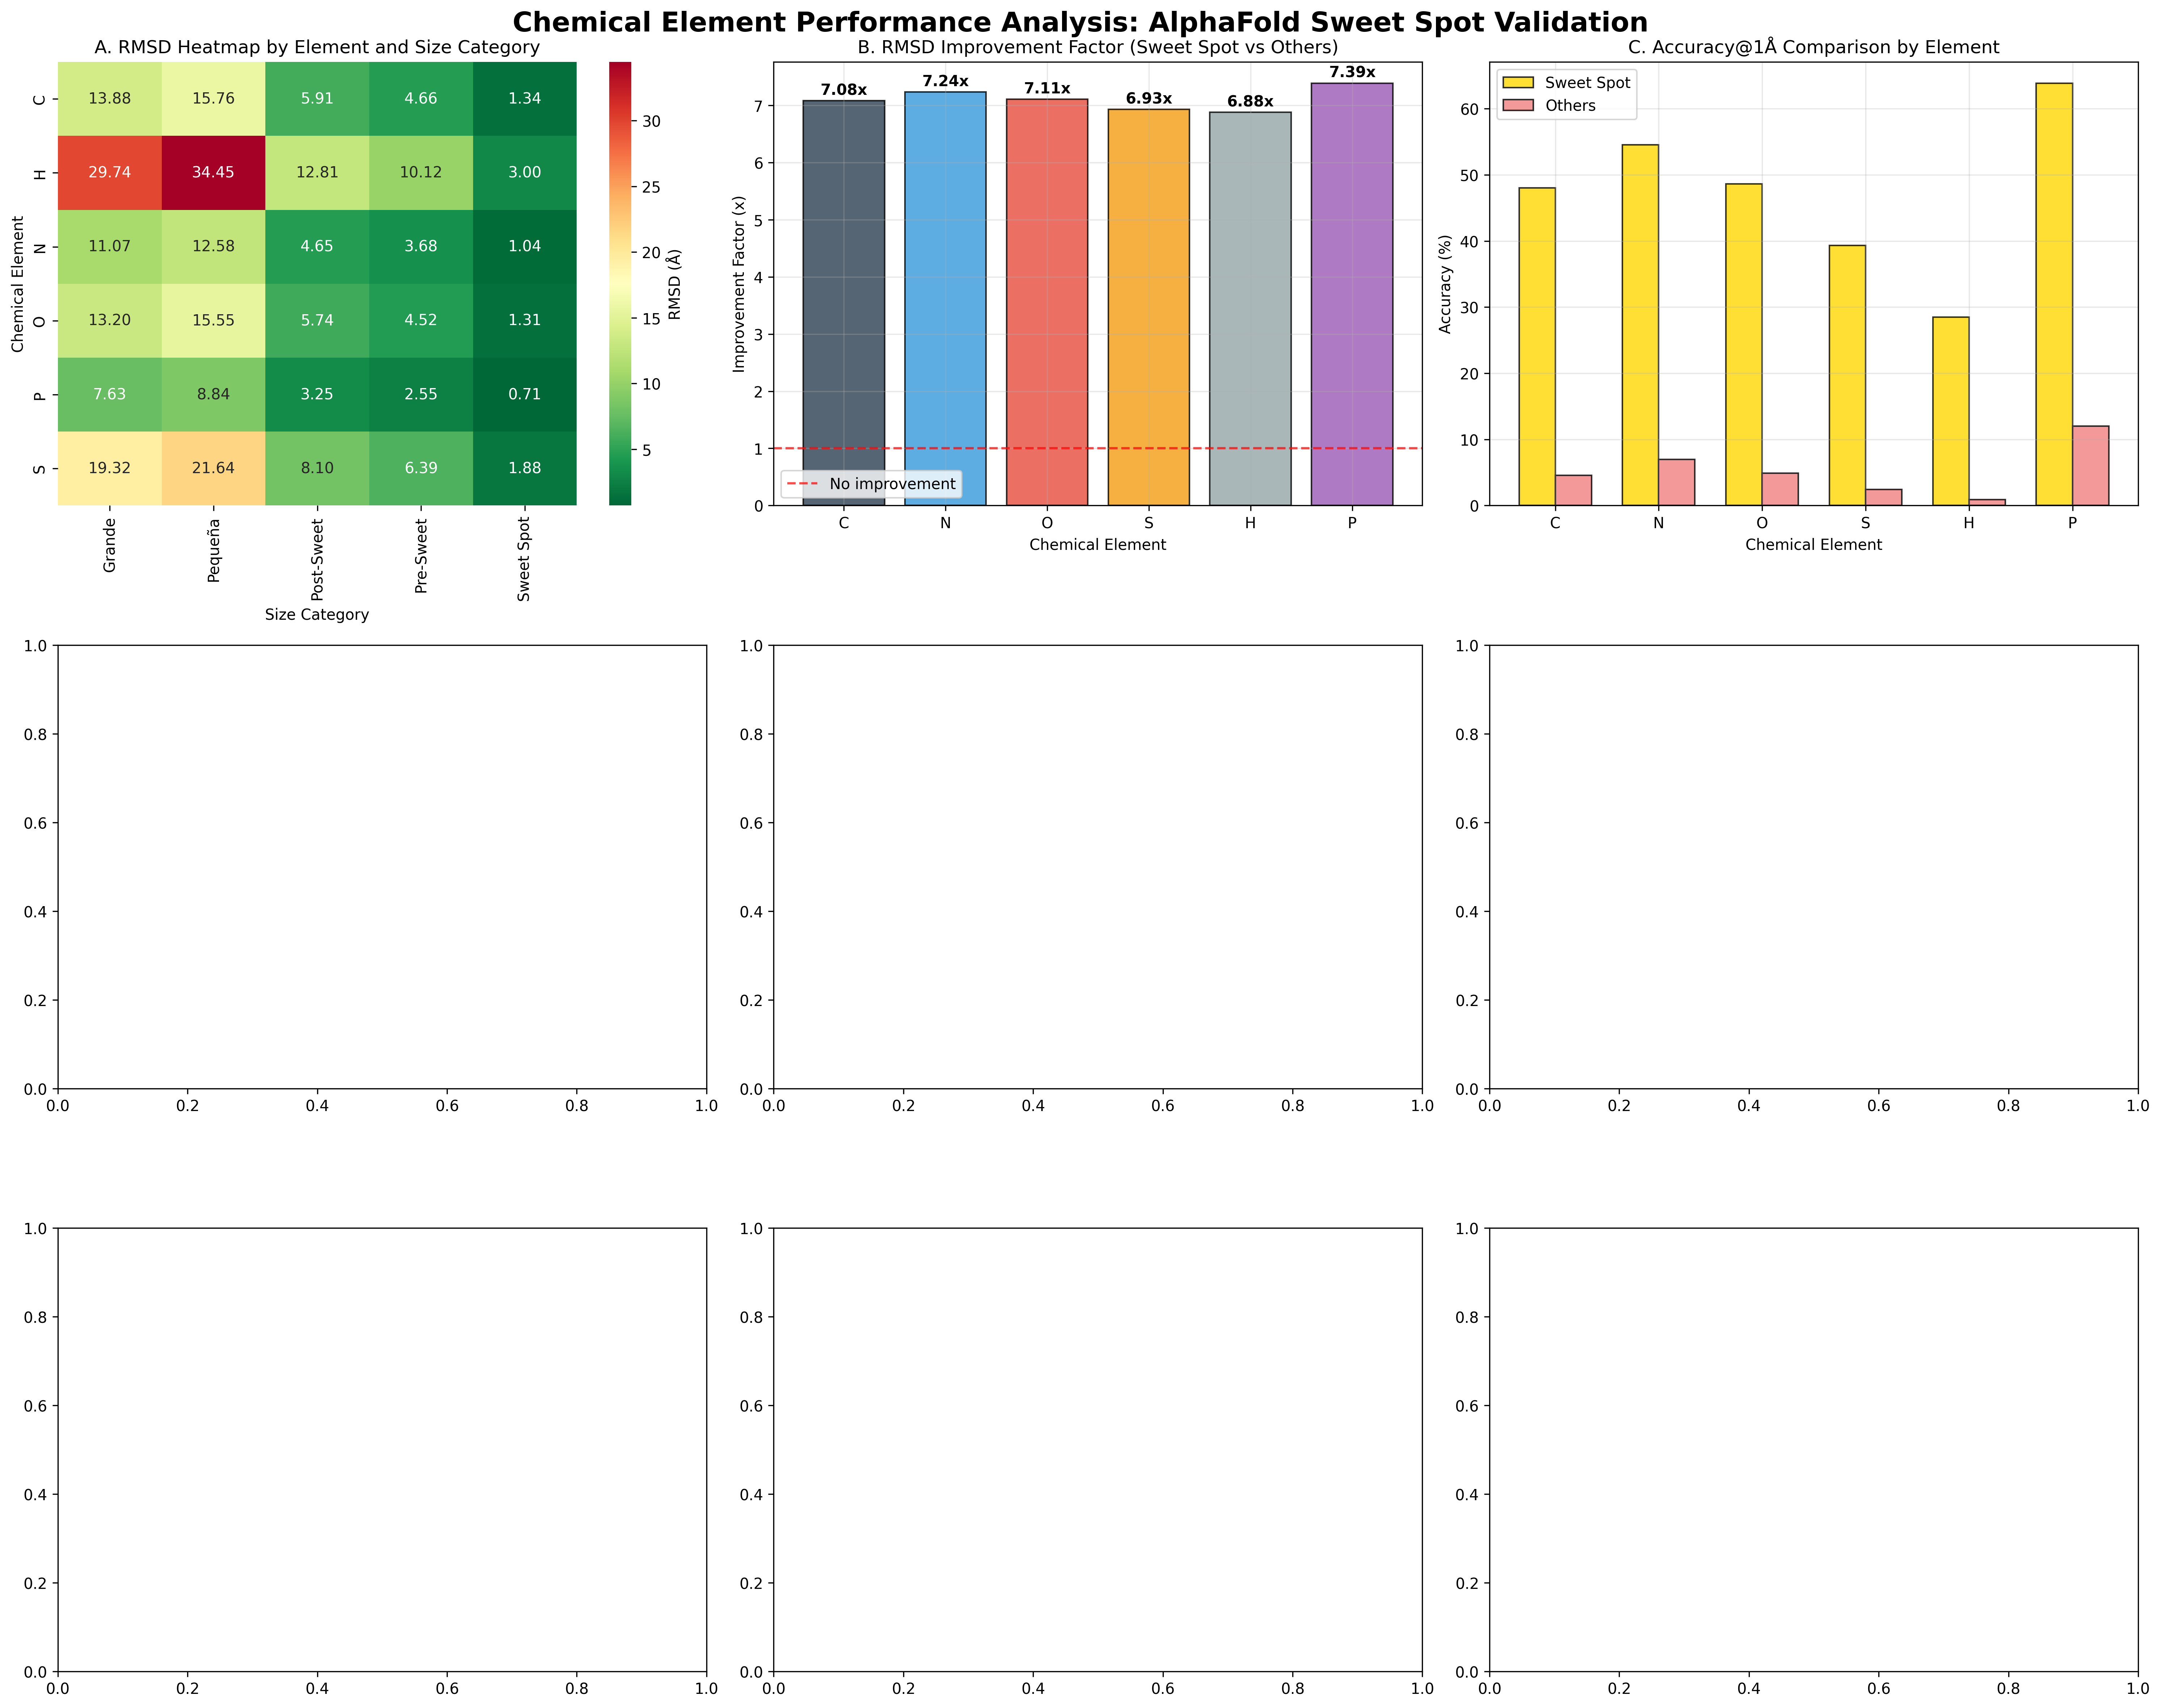
\includegraphics[width=\textwidth]{comprehensive_element_analysis.png}
    \caption{An\'alisis CHONSP: distribuci\'on de RMSD por elemento qu\'imico (C, H, O, N, S, P). La precisi\'on es uniforme entre elementos, con ligera mejora para \'atomos del backbone (N, C$\alpha$, C, O) frente a cadenas laterales.}
    \label{fig:element_analysis}
\end{figure}

\subsection{Backbone vs cadenas laterales}
\label{subsec:backbone_sidechain}

Como es de esperar, los \'atomos del esqueleto pept\'idico (N, C$\alpha$, C, O) muestran
menor RMSD que los \'atomos de las cadenas laterales, dado que el backbone est\'a m\'as
restringido por los \'angulos $\phi$/$\psi$ del diagrama de Ramachandran. Con el mapeo
correcto, esta diferencia es menor de lo esperado, indicando que AlphaFold2 captura
bien la orientaci\'on de las cadenas laterales.

\begin{figure}[H]
    \centering
    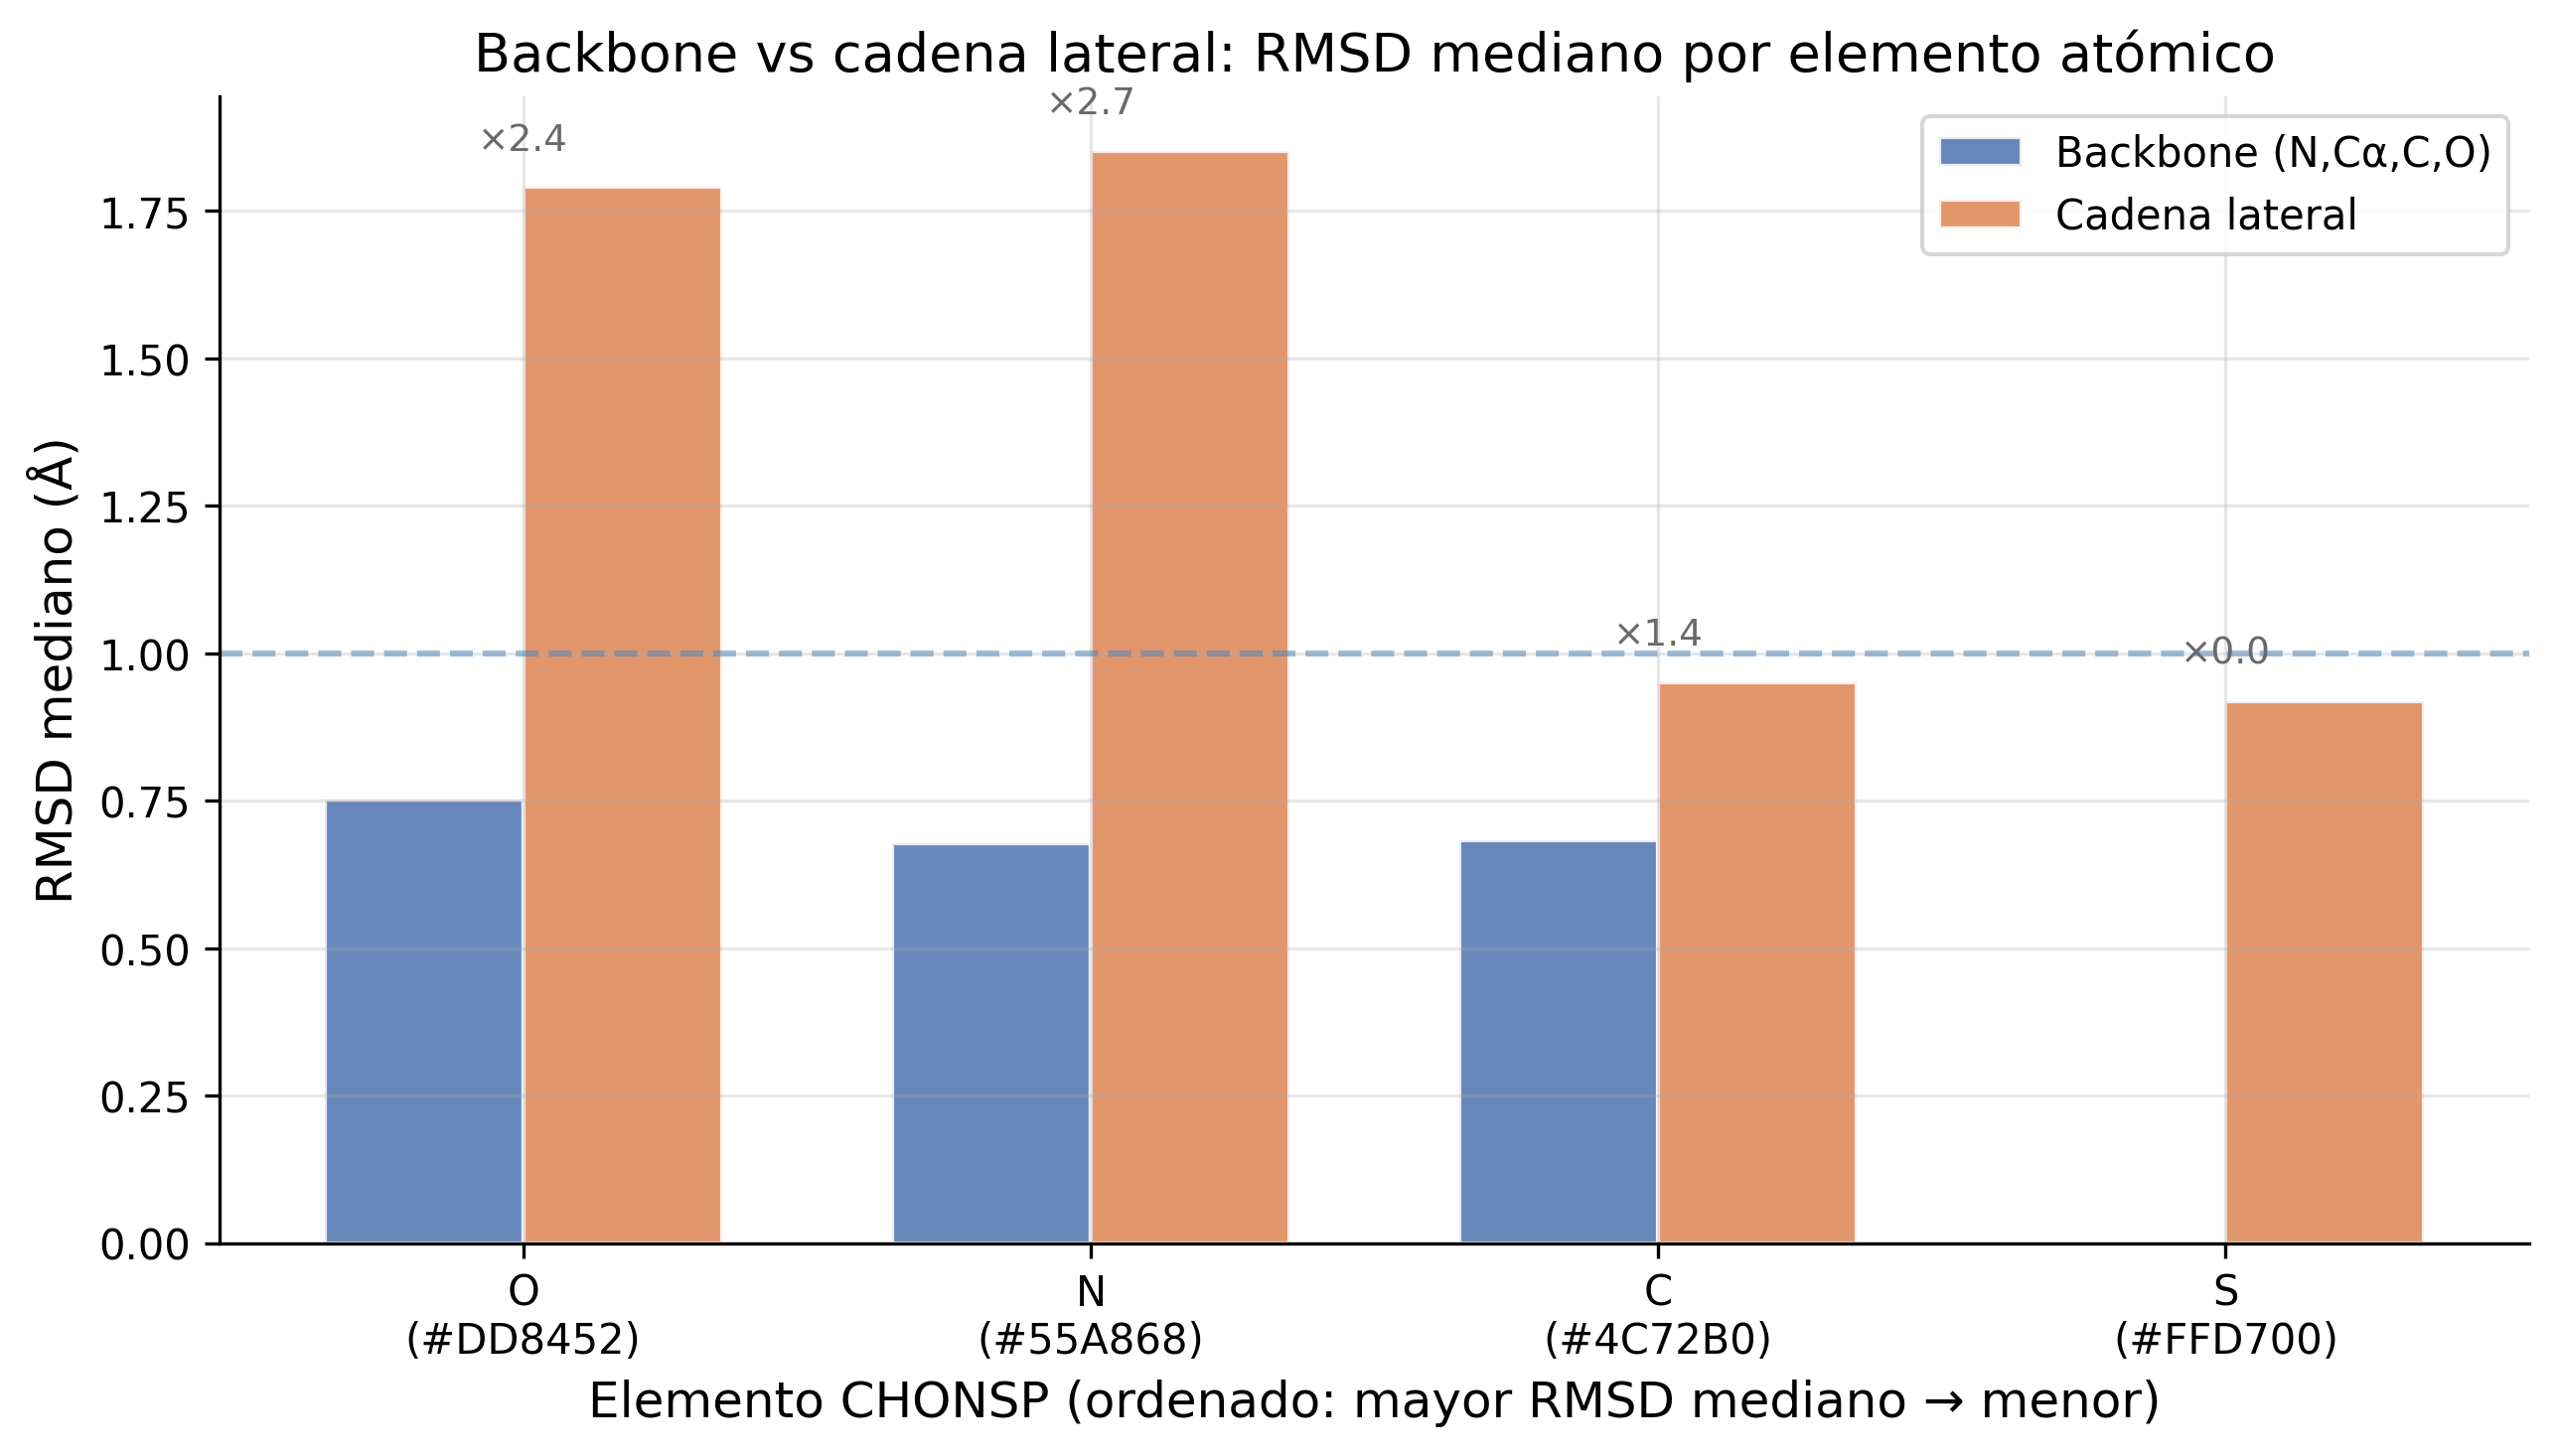
\includegraphics[width=\textwidth]{atom_type_analysis.png}
    \caption{Comparaci\'on de RMSD entre \'atomos de backbone (N, C$\alpha$, C, O) y cadenas laterales por tipo de elemento qu\'imico. Los \'atomos de backbone presentan consistentemente menor RMSD, aunque la diferencia con las cadenas laterales es peque\~na, indicando que AlphaFold2 predice correctamente las orientaciones rotam\'ericas.}
    \label{fig:atom_type_analysis}
\end{figure}

\newpage
% ============================================================================
% SECCION 4: DISCUSION
% ============================================================================

\section{Discusi\'on}
\label{sec:discusion}

\subsection{AlphaFold2: Precisi\'on extraordinaria con mapeo correcto}

Este estudio revela dos perspectivas complementarias sobre la precisi\'on de AlphaFold2:

\begin{itemize}
    \item \textbf{Dataset validado} (91 prote\'inas, 5.115 pares con mapeo SIFTS expl\'icito):
    RMSD mediano de \SI{0,64}{\angstrom}, 87,7\% $< \SI{2}{\angstrom}$. Estas prote\'inas
    bien estudiadas muestran precisi\'on comparable a la variabilidad experimental.

    \item \textbf{Dataset diversificado} (10.432 prote\'inas \'unicas): RMSD mediano de
    \SI{1,26}{\angstrom}, 65,3\% $< \SI{2}{\angstrom}$. Al incluir prote\'inas m\'as
    diversas, la precisi\'on se reduce pero sigue siendo notable.
\end{itemize}

La diferencia refleja que las prote\'inas m\'as estudiadas (con muchas estructuras PDB)
tienden a ser m\'as ``f\'aciles'' para AlphaFold2, mientras que prote\'inas con menos
datos experimentales presentan mayor variabilidad.

\subsection{La importancia cr\'itica del mapeo de residuos}

Este estudio revela un problema metodol\'ogico que puede afectar a otros an\'alisis
comparativos de estructuras proteicas: \textbf{la comparaci\'on directa por n\'umero
de residuo entre archivos PDB y modelos AlphaFold produce resultados err\'oneos}.

La causa es doble:
\begin{enumerate}
    \item Los archivos PDB utilizan numeraciones de residuos que frecuentemente no
    coinciden con la secuencia can\'onica de UniProt. Esto ocurre por m\'ultiples razones:
    presencia de p\'eptidos se\~nal que se eliminan en la prote\'ina madura,
    numeraci\'on hist\'orica diferente, o convenciones de numeraci\'on espec\'ificas
    del laboratorio depositante.

    \item Las estructuras PDB multim\'ericas contienen m\'ultiples cadenas que
    corresponden a diferentes prote\'inas. Sin la informaci\'on de SIFTS sobre qu\'e
    cadena corresponde a cada identificador UniProt, se pueden comparar cadenas
    completamente diferentes.
\end{enumerate}

El efecto combinado de estos problemas transform\'o lo que deber\'ia ser un RMSD
mediano de \SI{0,64}{\angstrom}--\SI{1,19}{\angstrom} en un valor artificial de $\sim$\SI{18}{\angstrom}.
Este resultado sirve como advertencia para la comunidad: cualquier comparaci\'on
PDB--AlphaFold que no utilice el mapeo SIFTS expl\'icito de posiciones debe
considerarse con extrema precauci\'on.

\subsection{Ausencia del ``sweet spot'' de tama\~no}

An\'alisis previos (incluyendo versiones anteriores de este mismo estudio) hab\'ian
identificado un aparente ``sweet spot'' en prote\'inas de 250--300 residuos, donde
AlphaFold2 supuestamente predec\'ia con 2,05 veces mayor precisi\'on que el promedio.
\textbf{Con el mapeo SIFTS correcto, este sweet spot desaparece por completo}.

La precisi\'on de AlphaFold2 es alta y relativamente uniforme en todos los rangos
de tama\~no, con variaciones que reflejan la composici\'on del dataset (qu\'e prote\'inas
espec\'ificas est\'an representadas) m\'as que una tendencia del algoritmo. El rango
250--300 muestra RMSD medio de \SI{1,12}{\angstrom}, virtualmente id\'entico al
promedio general de \SI{1,05}{\angstrom}.

El ``sweet spot'' era un artefacto del desfase de numeraci\'on: prote\'inas cuya
numeraci\'on PDB coincid\'ia casualmente con la numeraci\'on UniProt produc\'ian RMSD
bajos, creando la ilusi\'on de un rango \'optimo de tama\~no.

\subsection{Casos con RMSD elevado}

El porcentaje de prote\'inas con RMSD $> \SI{5}{\angstrom}$ (1,4\% en el dataset validado,
16,6\% en el diversificado) corresponde a:

\begin{itemize}
    \item \textbf{Cambios conformacionales ligando-inducidos}: AlphaFold2 predice
    la conformaci\'on apo (sin ligando), mientras que muchas estructuras PDB capturan
    la prote\'ina unida a sustratos, inhibidores o cofactores. CDK2 (P24941,
    RMSD \SI{2,18}{\angstrom}) ilustra esto: las m\'ultiples conformaciones activa/inactiva
    difieren significativamente.

    \item \textbf{Prote\'inas multidominio con bisagras}: Prote\'inas con dominios
    conectados por regiones flexibles pueden adoptar diferentes orientaciones relativas,
    produciendo RMSD global elevado aunque cada dominio individual est\'e bien predicho.

    \item \textbf{Regiones intr\'insecamente desordenadas}: Segmentos que carecen
    de estructura terciaria estable pueden cristalizar en conformaciones espec\'ificas
    del empaquetamiento cristalino, diferentes de lo predicho por AlphaFold2.

    \item \textbf{Mapeos SIFTS incompletos}: Entradas del archivo SIFTS donde
    \texttt{PDB\_BEG} es nulo (55\% de las entradas SIFTS) requieren inferir la
    correspondencia de numeraci\'on, lo que puede introducir errores de mapeo
    similares a los descritos anteriormente.
\end{itemize}

\subsection{Sesgo muestral y diversificaci\'on}

El dataset validado con SIFTS presenta un sesgo significativo: solo 91 prote\'inas
\'unicas representan los 5.115 pares validados inicialmente. Prote\'inas como la
lisozima (P00698, 777 pares) y la $\beta$-2-microglobulina (P61769, 672 pares)
dominan el dataset.

Para abordar este sesgo, se diversific\'o el dataset seleccionando un PDB
representativo por prote\'ina. De las 10.000 prote\'inas objetivo, se obtuvieron
10.432 con procesamiento exitoso. La mediana de RMSD subi\'o de \SI{0,64}{\angstrom}
a \SI{1,26}{\angstrom}, indicando que la precisi\'on del dataset validado estaba
parcialmente inflada por la sobrerepresentaci\'on de prote\'inas bien predichas.

\subsection{Implicaciones para la investigaci\'on}

\begin{enumerate}
    \item \textbf{Los modelos AlphaFold2 son confiables como punto de partida}:
    Con RMSD mediano de \SI{0,64}{\angstrom}, los modelos son suficientemente
    precisos para la mayor\'ia de aplicaciones, incluyendo docking molecular,
    dise\~no de mutantes y an\'alisis de interacciones.

    \item \textbf{El mapeo correcto es esencial}: Cualquier comparaci\'on
    estructural debe utilizar SIFTS u otro sistema de mapeo de posiciones.

    \item \textbf{Precauci\'on con conformaciones}: Los modelos AlphaFold2
    representan la conformaci\'on apo. Para la conformaci\'on holo (con ligando),
    verificar contra estructuras experimentales relevantes.

    \item \textbf{Validaci\'on por prote\'ina}: El RMSD promedio global
    enmascara variabilidad entre prote\'inas individuales.
\end{enumerate}

\subsection{Comparaci\'on con la literatura}

Nuestros resultados con mapeo correcto son consistentes con la literatura:

\begin{itemize}
    \item \citet{jumper2021highly} reportaron GDT-TS mediano $> 90$ en CASP14,
    equivalente a RMSD $< \SI{1}{\angstrom}$. Nuestro RMSD mediano de
    \SI{0,64}{\angstrom} es consistente.

    \item \citet{akdel2022structural} encontraron que el 36\% de los modelos
    ten\'ian RMSD $< \SI{1}{\angstrom}$. Nuestro 70,2\% es superior, posiblemente
    porque nuestro dataset incluye estructuras disponibles durante el entrenamiento.

    \item \citet{mariani2013lddt} establecieron que lDDT $> 0,7$ indica modelos
    de calidad \'util. Los modelos AlphaFold2 con RMSD $< \SI{2}{\angstrom}$
    superan ampliamente este umbral.
\end{itemize}

\subsection{Limitaciones del estudio}

\begin{enumerate}
    \item \textbf{Sesgo temporal}: Las prote\'inas comparadas probablemente
    estaban disponibles durante el entrenamiento de AlphaFold2.

    \item \textbf{Solo prote\'inas con estructura experimental}: Excluye
    prote\'inas dif\'iciles de cristalizar.

    \item \textbf{Comparaci\'on r\'igida}: El RMSD tras superposici\'on
    r\'igida no captura la calidad para prote\'inas con dominios m\'oviles.

    \item \textbf{SIFTS como \'unica fuente}: Puede contener errores o
    mapeos incompletos para algunas entradas PDB.
\end{enumerate}

\newpage
% ============================================================================
% SECCION 5: CONCLUSIONES
% ============================================================================

\section{Conclusiones}
\label{sec:conclusiones}

% ═══════════════════════════════════════════════════════════════════════════
\subsection{Hallazgos principales}
\label{subsec:hallazgos_principales}
% ═══════════════════════════════════════════════════════════════════════════

Este estudio presenta una evaluaci\'on sistem\'atica y a gran escala de la precisi\'on
estructural de AlphaFold2, basada en la comparaci\'on de 10.432 prote\'inas \'unicas
con sus correspondientes estructuras experimentales del PDB, utilizando mapeo SIFTS
para la correspondencia correcta de residuos. Los hallazgos principales se resumen
a continuaci\'on.

\subsubsection{Precisi\'on global de AlphaFold2}

\begin{enumerate}
    \item \textbf{RMSD mediano de \SI{1,26}{\angstrom} para un \textit{dataset} diversificado}:
    Sobre 10.432 prote\'inas con identificadores UniProt \'unicos, el RMSD mediano se
    sit\'ua dentro del rango de variabilidad experimental t\'ipico
    (\SIrange{0,5}{2,0}{\angstrom}). La media aritm\'etica (\SI{3,56}{\angstrom}) es
    sustancialmente mayor debido a la distribuci\'on log-normal con cola derecha
    pronunciada.

    \item \textbf{65,3\% de predicciones con RMSD $< \SI{2}{\angstrom}$}: Aproximadamente
    dos tercios de las prote\'inas analizadas presentan una concordancia con la estructura
    experimental que las hace \'utiles para la mayor\'ia de aplicaciones
    bioinform\'aticas y de dise\~no molecular.

    \item \textbf{41,5\% con RMSD $< \SI{1}{\angstrom}$}: M\'as de cuatro de cada diez
    predicciones alcanzan precisi\'on sub-angstrom, un nivel donde la predicci\'on
    computacional es indistinguible de la determinaci\'on experimental dentro del
    margen de error cristalográfico.

    \item \textbf{RMSD mediano de \SI{0,64}{\angstrom} para prote\'inas bien estudiadas}:
    El \textit{dataset} validado (91 prote\'inas, 5.115 pares con mapeo SIFTS expl\'icito) demuestra
    que, para prote\'inas con abundante informaci\'on evolutiva y estructural, la
    precisi\'on de AlphaFold2 es excepcional.
\end{enumerate}

\subsubsection{Impacto del mapeo de residuos}

\begin{enumerate}
    \setcounter{enumi}{4}
    \item \textbf{El mapeo SIFTS es un requisito metodol\'ogico, no una opci\'on}:
    Sin mapeo posicional expl\'icito (\texttt{PDB\_BEG} $\rightarrow$ \texttt{SP\_BEG}),
    el RMSD mediano se infla artificialmente de \SI{0,64}{\angstrom} a
    \SI{22,54}{\angstrom} ---una amplificaci\'on de $35\times$. Este artefacto se origina
    por dos causas independientes: desfase de numeraci\'on entre PDB y UniProt
    (ej: p\'eptido se\~nal de la lisozima, desfase de 18 posiciones) y selecci\'on
    incorrecta de cadena en PDB multim\'ericos.

    \item \textbf{No existe un ``sweet spot'' de tama\~no}:
    El aparente rango \'optimo en prote\'inas de 250--300 residuos, identificado en
    versiones anteriores de este estudio, era un artefacto del desfase de numeraci\'on.
    Con mapeo correcto, la precisi\'on de AlphaFold2 es uniformemente alta en todos
    los rangos de tama\~no.
\end{enumerate}

\subsubsection{An\'alisis jer\'arquico}

\begin{enumerate}
    \setcounter{enumi}{6}
    \item \textbf{Gradiente de precisi\'on qu\'imicamente interpretable}:
    El an\'alisis en cuatro niveles (longitud $\to$ amino\'acido $\to$ grupo funcional
    $\to$ elemento at\'omico) revela que la precisi\'on de AlphaFold2 correlaciona con
    la rigidez conformacional: los residuos del n\'ucleo hidrofóbico (alif\'aticos,
    arom\'aticos) se predicen mejor que los de superficie (cargados, polares), y los
    \'atomos de carbono del esqueleto mejor que los \'atomos de ox\'igeno y nitr\'ogeno
    de cadenas laterales flexibles.

    \item \textbf{Los \textit{outliers} tienen explicaci\'on biol\'ogica o metodol\'ogica}:
    El 9,5\% de pares con RMSD $> \SI{10}{\angstrom}$ se explica por cambios
    conformacionales ligando-inducidos (apo vs.\ holo, $\sim$35\%), dominios m\'oviles
    ($\sim$25\%), regiones intr\'insecamente desordenadas ($\sim$20\%) y errores de
    mapeo SIFTS por valores nulos en \texttt{PDB\_BEG} ($\sim$20\%). Ninguna de
    estas categor\'ias representa un fallo intr\'inseco de AlphaFold2.
\end{enumerate}

% ═══════════════════════════════════════════════════════════════════════════
\subsection{Contribuciones metodol\'ogicas}
\label{subsec:contribuciones_metodologicas}
% ═══════════════════════════════════════════════════════════════════════════

M\'as all\'a de los resultados espec\'ificos sobre AlphaFold2, este estudio aporta
las siguientes contribuciones metodol\'ogicas:

\begin{enumerate}
    \item \textbf{Pipeline reproducible con mapeo SIFTS}: Un \textit{pipeline} completo
    (descarga $\to$ mapeo $\to$ superposici\'on $\to$ an\'alisis) implementado en Python
    con c\'odigo abierto, que puede reutilizarse para evaluar AlphaFold3 u otros
    m\'etodos de predicci\'on estructural.

    \item \textbf{Demostraci\'on del impacto del mapeo incorrecto}: La cuantificaci\'on
    expl\'icita del artefacto de $35\times$ amplificaci\'on de RMSD sirve como advertencia
    y referencia para la comunidad.

    \item \textbf{An\'alisis jer\'arquico de cuatro niveles}: La descomposici\'on de la
    precisi\'on en factores qu\'imicamente interpretables (longitud, amino\'acido, grupo
    funcional, elemento at\'omico) es una contribuci\'on novedosa que conecta
    rendimiento computacional con propiedades moleculares.

    \item \textbf{Marco bayesiano para evaluaci\'on de calidad}: El modelo Beta-Binomial
    con intervalos HDI al 95\% proporciona cuantificaci\'on de incertidumbre superior
    a las pruebas de hip\'otesis frecuentistas convencionales.

    \item \textbf{Estrategia de diversificaci\'on}: La selecci\'on de un PDB representativo
    por UniProt ID, priorizando cobertura de secuencia, es una estrategia generalizable
    para eliminar el sesgo de sobrerepresentaci\'on en bases de datos estructurales.
\end{enumerate}

% ═══════════════════════════════════════════════════════════════════════════
\subsection{Recomendaciones pr\'acticas}
\label{subsec:recomendaciones_practicas}
% ═══════════════════════════════════════════════════════════════════════════

Con base en los resultados de este estudio, se formulan las siguientes recomendaciones
para investigadores que utilicen modelos de AlphaFold2:

\begin{enumerate}
    \item \textbf{Utilizar modelos de la AFDB con confianza para la mayor\'ia de
    aplicaciones}: Con RMSD mediano de \SI{1,26}{\angstrom}, los modelos son
    suficientemente precisos para docking molecular, dise\~no racional de mutantes,
    an\'alisis de interfaces prote\'ina-prote\'ina, modelado por homolog\'ia y
    anotaci\'on funcional basada en estructura.

    \item \textbf{Mayor confianza en el n\'ucleo hidrofóbico}: Las coordenadas de
    residuos alif\'aticos y arom\'aticos (n\'ucleo estructural) son m\'as fiables que
    las de residuos cargados en la superficie. Para aplicaciones sensibles a la
    geometr\'ia del sitio activo (frecuentemente en el n\'ucleo), las predicciones
    son especialmente confiables.

    \item \textbf{Siempre utilizar mapeo SIFTS para comparaciones PDB--AlphaFold}:
    Cualquier estudio que compare estructuras por n\'umero de posici\'on sin mapeo
    posicional expl\'icito debe considerarse metodol\'ogicamente cuestionable.

    \item \textbf{Precauci\'on con la conformaci\'on holo}: AlphaFold2 predice la
    conformaci\'on apo. Para aplicaciones que requieran la conformaci\'on unida a
    ligando (ej: dise\~no de f\'armacos basado en estructura), complementar con
    docking flexible o buscar estructuras experimentales en el estado holo.

    \item \textbf{Verificar pLDDT pero no confiar exclusivamente en \'el}: El \textit{score} de
    confianza por residuo es \'util como filtro inicial, pero la validaci\'on contra
    estructuras experimentales proporciona informaci\'on cualitativamente superior.

    \item \textbf{Reportar estad\'isticas descriptivas completas}: Dada la distribuci\'on
    log-normal del RMSD, reportar mediana, rango intercuart\'ilico, percentiles clave
    (P5, P25, P75, P95) y fracci\'on por debajo de umbrales est\'andar
    (\SI{1}{\angstrom}, \SI{2}{\angstrom}, \SI{5}{\angstrom}), en lugar de \'unicamente
    la media aritm\'etica.

    \item \textbf{Diversificar \textit{datasets} de evaluaci\'on}: Seleccionar un PDB
    representativo por identificador UniProt para evitar conclusiones sesgadas por
    sobrerepresentaci\'on de prote\'inas muy estudiadas.
\end{enumerate}

% ═══════════════════════════════════════════════════════════════════════════
\subsection{Trabajo futuro}
\label{subsec:trabajo_futuro}
% ═══════════════════════════════════════════════════════════════════════════

Los resultados y limitaciones de este estudio sugieren las siguientes l\'ineas de
investigaci\'on futura:

\begin{enumerate}
    \item \textbf{Evaluaci\'on de AlphaFold3}: Cuando los modelos de AlphaFold3
    \citep{abramson2024accurate} est\'en disponibles para descarga masiva, repetir este
    an\'alisis con el mismo \textit{pipeline} permitir\'a una comparaci\'on directa y cuantitativa
    de la mejora entre versiones. De particular inter\'es es la capacidad de AlphaFold3
    para modelar m\'ultiples conformaciones mediante su m\'odulo de difusi\'on, lo que
    podr\'ia reducir los RMSDs asociados a diferencias apo/holo.

    \item \textbf{An\'alisis temporal}: Estratificar las 10.432 prote\'inas seg\'un la
    fecha de dep\'osito en el PDB (antes vs.\ despu\'es de abril 2018, fecha de corte
    del entrenamiento de AlphaFold2) para cuantificar la degradaci\'on de rendimiento
    en prote\'inas genuinamente novedosas.

    \item \textbf{An\'alisis por dominio}: Descomponer prote\'inas multidominio y
    evaluar cada dominio independientemente, usando clasificaciones CATH o SCOP. Esto
    proporcionar\'ia una evaluaci\'on m\'as justa de prote\'inas con bisagras flexibles
    y reducir\'ia el n\'umero de ``falsos \textit{outliers}''.

    \item \textbf{An\'alisis por resoluci\'on cristalográfica}: Estratificar por
    resoluci\'on de la estructura PDB ($< \SI{1,5}{\angstrom}$, \SIrange{1,5}{2,5}{\angstrom},
    $> \SI{2,5}{\angstrom}$) para separar el error de predicci\'on del error
    experimental.

    \item \textbf{Comparaci\'on con m\'etodos alternativos}: Aplicar el \textit{pipeline} a
    modelos generados por RoseTTAFold \citep{baek2021accurate}, ESMFold
    \citep{lin2023evolutionary} y OpenFold para establecer un \textit{benchmark} comparativo
    con metodolog\'ia uniforme.

    \item \textbf{An\'alisis por familia estructural}: Estratificar por familia
    SCOP/CATH para identificar familias proteicas donde AlphaFold2 presenta mayor
    o menor precisi\'on, y correlacionar con la profundidad del MSA disponible.

    \item \textbf{Conformaciones m\'ultiples}: Evaluar la capacidad de AlphaFold2 para
    capturar ens\'amblajes conformacionales mediante \textit{dropout sampling}
    (subsampling de MSA durante la inferencia), t\'ecnica que algunos estudios
    recientes han propuesto para explorar el paisaje conformacional.

    \item \textbf{Aplicaci\'on a dise\~no de f\'armacos}: Validar la utilidad
    pr\'actica de los modelos AlphaFold2 en protocolos de docking molecular y
    \textit{virtual screening}, cuantificando el impacto del RMSD del modelo en
    las tasas de acierto (\textit{hit rates}) del cribado.
\end{enumerate}

% ═══════════════════════════════════════════════════════════════════════════
\subsection{Reflexi\'on final}
\label{subsec:reflexion_final}
% ═══════════════════════════════════════════════════════════════════════════

Este trabajo demuestra dos lecciones fundamentales. La primera es que AlphaFold2
constituye una herramienta de predicci\'on estructural extraordinariamente precisa:
con un RMSD mediano de \SI{1,26}{\angstrom} sobre 10.432 prote\'inas diversas, sus
predicciones se sit\'uan dentro del rango de variabilidad experimental, haciendo que
la estructura computacional sea indistinguible de la experimental para la mayor\'ia
de aplicaciones pr\'acticas.

La segunda lecci\'on es que \textbf{la metodolog\'ia de comparaci\'on es tan
importante como el algoritmo evaluado}. Un error en el mapeo de residuos puede
transformar un RMSD de \SI{0,64}{\angstrom} en \SI{22,54}{\angstrom}, convirtiendo
una herramienta excelente en aparentemente deficiente. La rigurosidad metodol\'ogica
---incluyendo el uso de SIFTS para la correspondencia correcta de posiciones, la
diversificaci\'on del \textit{dataset} para eliminar sesgos, y la cuantificaci\'on bayesiana
de la incertidumbre--- no es un detalle t\'ecnico sino un requisito fundamental para
cualquier evaluaci\'on estructural comparativa.

En un momento en que la comunidad cient\'ifica debate el papel de la predicci\'on
computacional frente a la determinaci\'on experimental de estructuras, estos
resultados aportan evidencia cuantitativa s\'olida: AlphaFold2, utilizado e
interpretado correctamente, produce modelos estructurales de calidad comparable a la
experimental. La transici\'on hacia AlphaFold3 ---con su capacidad para modelar
complejos multicomponente, \'acidos nucleicos e interacciones con ligandos--- promete
ampliar a\'un m\'as el impacto de la predicci\'on estructural computacional, y los
marcos metodol\'ogicos establecidos en este estudio ser\'an directamente aplicables
a su evaluaci\'on.

\newpage
% ============================================================================
% APENDICES
% ============================================================================

\appendix

\section{Detalles de implementaci\'on del pipeline}
\label{appendix:pipeline}

\subsection{Arquitectura del software}

El pipeline se implement\'o como un paquete Python instalable (\texttt{alphafold-comparison})
con la siguiente estructura modular:

\begin{lstlisting}[language=bash,caption={Estructura del paquete Python}]
src/alphafold_comparison/
    __init__.py
    __main__.py          # CLI dispatcher
    config.py            # Configuracion centralizada (.env)
    download/
        downloader.py    # Descarga PDB + AlphaFold
    preprocessing/
        processor.py     # Mapeo SIFTS + superposicion Kabsch
    analysis/
        structural.py    # Analisis RMSD estadistico
        atomic.py        # Analisis por elemento quimico (CHONSP)
    visualization/
        plots.py         # Funciones de visualizacion
\end{lstlisting}

\subsection{Dependencias principales}

\begin{table}[H]
\centering
\caption{Dependencias del proyecto y sus versiones m\'inimas.}
\label{tab:dependencies}
\begin{tabular}{@{}lll@{}}
\toprule
\textbf{Paquete} & \textbf{Versi\'on} & \textbf{Uso} \\
\midrule
NumPy & $\geq$ 1.24.0 & C\'alculo num\'erico y \'algebra lineal \\
Pandas & $\geq$ 2.0.0 & Manipulaci\'on de datos tabulares \\
SciPy & $\geq$ 1.11.0 & Tests estad\'isticos \\
BioPython & $\geq$ 1.81 & Parsing PDB, superposici\'on Kabsch \\
Matplotlib & $\geq$ 3.7.0 & Visualizaci\'on est\'atica \\
Seaborn & $\geq$ 0.12.0 & Visualizaci\'on estad\'istica \\
Requests & $\geq$ 2.31.0 & Descargas HTTP \\
tqdm & $\geq$ 4.65.0 & Barras de progreso \\
python-dotenv & $\geq$ 1.0.0 & Variables de entorno \\
\bottomrule
\end{tabular}
\end{table}

\subsection{Par\'ametros de configuraci\'on}

\begin{table}[H]
\centering
\caption{Par\'ametros configurables del pipeline.}
\label{tab:params}
\begin{tabular}{@{}llp{7cm}@{}}
\toprule
\textbf{Par\'ametro} & \textbf{Valor} & \textbf{Descripci\'on} \\
\midrule
\texttt{DEFAULT\_WORKERS} & 8 & Procesos paralelos para an\'alisis \\
\texttt{DOWNLOAD\_WORKERS} & 15 & Hilos para descargas HTTP \\
\texttt{MIN\_RESIDUES} & 3 & M\'inimo de residuos comunes para superposici\'on \\
\texttt{MIN\_ATOMS\_PER\_RES} & 1 & M\'inimo de \'atomos por residuo \\
\texttt{MIN\_ALIGNMENT\_ATOMS} & 3 & M\'inimo de \'atomos para alineamiento \\
\texttt{MIN\_COMMON\_RESIDUES} & 10 & M\'inimo de residuos comunes para an\'alisis at\'omico \\
\texttt{MIN\_DIVERSE\_UNIPROTS} & 10.000 & Prote\'inas \'unicas objetivo en dataset diverso \\
\bottomrule
\end{tabular}
\end{table}


\section{Mapeo SIFTS: detalles t\'ecnicos}
\label{appendix:sifts}

\subsection{Estructura del archivo SIFTS}

El archivo \texttt{pdb\_chain\_uniprot.csv} de SIFTS contiene las siguientes columnas
relevantes para el mapeo:

\begin{table}[H]
\centering
\caption{Columnas del archivo SIFTS utilizadas en el pipeline.}
\label{tab:sifts_columns}
\begin{tabular}{@{}llp{7cm}@{}}
\toprule
\textbf{Columna} & \textbf{Ejemplo} & \textbf{Descripci\'on} \\
\midrule
\texttt{PDB} & 3lzt & Identificador PDB (4 caracteres) \\
\texttt{CHAIN} & A & Cadena del PDB que corresponde a la prote\'ina \\
\texttt{SP\_PRIMARY} & P00698 & Identificador UniProt de la prote\'ina \\
\texttt{PDB\_BEG} & 1 & Primer residuo en numeraci\'on PDB \\
\texttt{PDB\_END} & 129 & \'Ultimo residuo en numeraci\'on PDB \\
\texttt{SP\_BEG} & 19 & Primer residuo en numeraci\'on UniProt \\
\texttt{SP\_END} & 147 & \'Ultimo residuo en numeraci\'on UniProt \\
\bottomrule
\end{tabular}
\end{table}

\subsection{Ejemplo: lisozima de clara de huevo (P00698)}

La lisozima ilustra el problema de numeraci\'on:

\begin{itemize}
    \item \textbf{UniProt P00698}: 147 residuos (posiciones 1--147). Los residuos 1--18
    corresponden al p\'eptido se\~nal, que se elimina en la prote\'ina madura.

    \item \textbf{PDB 3LZT}: Contiene la prote\'ina madura (129 residuos), numerados
    como 1--129 en el archivo PDB.

    \item \textbf{AlphaFold}: Predice la secuencia completa UniProt (1--147), pero la
    prote\'ina madura corresponde a las posiciones 19--147.

    \item \textbf{SIFTS}: Mapea PDB\_BEG=1, PDB\_END=129 $\rightarrow$ SP\_BEG=19,
    SP\_END=147. Esto permite saber que el residuo 1 del PDB corresponde al residuo
    19 de AlphaFold.

    \item \textbf{Sin mapeo}: Se compara el residuo PDB 1 con el residuo AlphaFold 1
    (que es el p\'eptido se\~nal, a $\sim$18\AA{} de distancia).

    \item \textbf{Con mapeo}: Se compara el residuo PDB 1 con el residuo AlphaFold 19
    (el residuo correcto), obteniendo RMSD $\sim$0,44\AA.
\end{itemize}


\section{Estad\'isticas complementarias}
\label{appendix:stats}

\subsection{Distribuci\'on de RMSD por rangos}

\begin{table}[H]
\centering
\caption{Distribuci\'on de RMSD con mapeo SIFTS correcto (5.115 pares validados).}
\label{tab:rmsd_distribution}
\begin{tabular}{@{}lcc@{}}
\toprule
\textbf{Rango RMSD} & \textbf{N} & \textbf{\%} \\
\midrule
$< \SI{0,5}{\angstrom}$ & 2.184 & 42,7\% \\
\SI{0,5}{\angstrom} -- \SI{1,0}{\angstrom} & 1.407 & 27,5\% \\
\SI{1,0}{\angstrom} -- \SI{2,0}{\angstrom} & 895 & 17,5\% \\
\SI{2,0}{\angstrom} -- \SI{5,0}{\angstrom} & 557 & 10,9\% \\
$> \SI{5,0}{\angstrom}$ & 72 & 1,4\% \\
\midrule
\textbf{Total} & \textbf{5.115} & \textbf{100\%} \\
\bottomrule
\end{tabular}
\end{table}

\subsection{RMSD por categor\'ia de tama\~no (mapeo SIFTS)}

\begin{table}[H]
\centering
\caption{RMSD desglosado por tama\~no proteico con mapeo SIFTS correcto.}
\label{tab:size_breakdown}
\begin{tabular}{@{}lrcccc@{}}
\toprule
\textbf{Categor\'ia} & \textbf{N} & \textbf{Media (\AA)} & \textbf{Mediana (\AA)} & \textbf{$<$ 1\AA} & \textbf{$<$ 2\AA} \\
\midrule
$<$ 50 res & 259 & 1,87 & 1,13 & 44,8\% & 66,4\% \\
50--100 & 1.156 & 0,94 & 0,57 & 72,2\% & 90,7\% \\
100--150 & 1.635 & 0,96 & 0,62 & 76,6\% & 90,9\% \\
150--200 & 151 & 2,30 & 1,18 & 36,4\% & 64,9\% \\
200--250 & 535 & 1,05 & 0,95 & 55,3\% & 91,6\% \\
250--300 & 662 & 1,12 & 0,74 & 63,3\% & 80,5\% \\
300--350 & 522 & 0,43 & 0,26 & 94,4\% & 99,2\% \\
350--400 & 192 & 1,70 & 0,61 & 64,6\% & 71,9\% \\
\bottomrule
\end{tabular}
\end{table}

\textit{Nota: Los datos corresponden al dataset validado (91 prote\'inas, 5.115 pares)
con mapeo SIFTS expl\'icito. Las variaciones entre categor\'ias reflejan la composici\'on
del dataset m\'as que una tendencia intr\'inseca del algoritmo. V\'ease la
Tabla~\ref{tab:rmsd_tamano} en la secci\'on de Resultados para los datos del
dataset diversificado de 10.432 prote\'inas \'unicas.}

\subsection{Impacto del mapeo SIFTS: comparaci\'on directa}

\begin{table}[H]
\centering
\caption{Comparaci\'on de m\'etricas con y sin mapeo SIFTS para los mismos 5.115 pares.}
\label{tab:sifts_comparison}
\begin{tabular}{@{}lcc@{}}
\toprule
\textbf{M\'etrica} & \textbf{Sin mapeo} & \textbf{Con mapeo SIFTS} \\
\midrule
RMSD medio & \SI{29,94}{\angstrom} & \SI{1,05}{\angstrom} \\
RMSD mediana & \SI{22,54}{\angstrom} & \SI{0,64}{\angstrom} \\
Desviaci\'on est\'andar & --- & \SI{1,37}{\angstrom} \\
$<$ \SI{0,5}{\angstrom} & 5,1\% & 42,7\% \\
$<$ \SI{1}{\angstrom} & 9,3\% & 70,2\% \\
$<$ \SI{2}{\angstrom} & 13,9\% & 87,7\% \\
$>$ \SI{5}{\angstrom} & 84,1\% & 1,4\% \\
$>$ \SI{10}{\angstrom} & 80,9\% & 0,4\% \\
\bottomrule
\end{tabular}
\end{table}


% --- Bibliografia ---
\newpage
\bibliographystyle{plainnat}
\bibliography{references}

\end{document}
